%% Note: Authors migrating a paper from PACMPL format to traditional
%% SIGPLAN proceedings format should change 'acmlarge' to
%% 'sigplan,10pt'.
%% For double-blind review submission, w/o CCS and ACM Reference (max submission space)
\documentclass[sigplan,review,anonymous]{acmart}\settopmatter{printfolios=true,printccs=false,printacmref=false}
%% For double-blind review submission, w/ CCS and ACM Reference
%\documentclass[sigplan,review,anonymous]{acmart}\settopmatter{printfolios=true}
%% For single-blind review submission, w/o CCS and ACM Reference (max submission space)
%\documentclass[sigplan,review]{acmart}\settopmatter{printfolios=true,printccs=false,printacmref=false}
%% For single-blind review submission, w/ CCS and ACM Reference
%\documentclass[sigplan,review]{acmart}\settopmatter{printfolios=true}
%% For final camera-ready submission, w/ required CCS and ACM Reference
%\documentclass[sigplan]{acmart}\settopmatter{}

\newcommand{\PAPER}{}
\newcommand{\either}[2]{#2}

%% Some recommended packages.
%\usepackage{booktabs}   %% For formal tables:
%                        %% http://ctan.org/pkg/booktabs
%\usepackage{subcaption} %% For complex figures with subfigures/subcaptions
%                        %% http://ctan.org/pkg/subcaption

\usepackage{esop-common}
\usepackage{infer-common}
\usepackage{quals-common}

\makeatletter\if@ACM@journal\makeatother
%% Journal information (used by PACMPL format)
%% Supplied to authors by publisher for camera-ready submission
\acmJournal{PACMPL}
\acmVolume{1}
\acmNumber{1}
\acmArticle{1}
\acmYear{2017}
\acmMonth{1}
\acmDOI{10.1145/nnnnnnn.nnnnnnn}
\startPage{1}
\else\makeatother
%% Conference information (used by SIGPLAN proceedings format)
%% Supplied to authors by publisher for camera-ready submission
\acmConference[PL'17]{ACM SIGPLAN Conference on Programming Languages}{January 01--03, 2017}{New York, NY, USA}
\acmYear{2017}
\acmISBN{978-x-xxxx-xxxx-x/YY/MM}
\acmDOI{10.1145/nnnnnnn.nnnnnnn}
\startPage{1}
\fi


%% Copyright information
%% Supplied to authors (based on authors' rights management selection;
%% see authors.acm.org) by publisher for camera-ready submission
\setcopyright{none}             %% For review submission
%\setcopyright{acmcopyright}
%\setcopyright{acmlicensed}
%\setcopyright{rightsretained}
%\copyrightyear{2017}           %% If different from \acmYear


%% Bibliography style
\bibliographystyle{ACM-Reference-Format}
%% Citation style
%% Note: author/year citations are required for papers published as an
%% issue of PACMPL.
%\citestyle{acmauthoryear}   %% For author/year citations



\begin{document}

%% Title information
%\title[Short Title]{Full Title}         %% [Short Title] is optional;
%                                        %% when present, will be used in
%                                        %% header instead of Full Title.
%\title{Dynamic Type Inference for Recursive Structural Types}
%\title{ from unit tests to generative tests and types}
%\title{Generating generative tests}
%\title{Generating generative tests, then types}
%\title{From tests, to generative tests and types, automatically}
%\title{Squash the work}
%\title{Squash the work: Generating useful optional types}
\title{Squash the work: Automatic annotations for untyped languages}
%\title{Generating useful types for optionally typed languages}
%\subtitle{Generating useful optional types}
%\subtitle{Ease the porting process}
%\titlenote{with title note}             %% \titlenote is optional;
%                                        %% can be repeated if necessary;
%                                        %% contents suppressed with 'anonymous'
%\subtitle{Subtitle}                     %% \subtitle is optional
%\subtitlenote{with subtitle note}       %% \subtitlenote is optional;
%                                        %% can be repeated if necessary;
%                                        %% contents suppressed with 'anonymous'


%% Author information
%% Contents and number of authors suppressed with 'anonymous'.
%% Each author should be introduced by \author, followed by
%% \authornote (optional), \orcid (optional), \affiliation, and
%% \email.
%% An author may have multiple affiliations and/or emails; repeat the
%% appropriate command.
%% Many elements are not rendered, but should be provided for metadata
%% extraction tools.

%% Author with single affiliation.
\author{Ambrose Bonnaire-Sergeant}
%\authornote{with author1 note}          %% \authornote is optional;
                                        %% can be repeated if necessary
%\orcid{nnnn-nnnn-nnnn-nnnn}             %% \orcid is optional
\affiliation{
  %\position{Position1}
  \department{Computer Science}              %% \department is recommended
  \institution{Indiana University}            %% \institution is required
  %\streetaddress{Street1 Address1}
  %\city{City1}
  %\state{State1}
  %\postcode{Post-Code1}
  \country{USA}
}
\email{abonnair@iu.edu}          %% \email is recommended

%% Author with two affiliations and emails.
\author{Sam Tobin-Hochstadt}
%\authornote{with author2 note}          %% \authornote is optional;
                                        %% can be repeated if necessary
%\orcid{nnnn-nnnn-nnnn-nnnn}             %% \orcid is optional
\affiliation{
  %\position{Position2a}
  \department{Computer Science}             %% \department is recommended
  \institution{Indiana University}           %% \institution is required
  %\streetaddress{Street2a Address2a}
  %\city{City2a}
  %\state{State2a}
  %\postcode{Post-Code2a}
  \country{USA}
}
\email{samth@iu.edu}         %% \email is recommended
%\affiliation{
%  \position{Position2b}
%  \department{Department2b}             %% \department is recommended
%  \institution{Institution2b}           %% \institution is required
%  \streetaddress{Street3b Address2b}
%  \city{City2b}
%  \state{State2b}
%  \postcode{Post-Code2b}
%  \country{Country2b}
%}
%\email{first2.last2@inst2b.org}         %% \email is recommended


%% Paper note
%% The \thanks command may be used to create a "paper note" ---
%% similar to a title note or an author note, but not explicitly
%% associated with a particular element.  It will appear immediately
%% above the permission/copyright statement.
%\thanks{with paper note}                %% \thanks is optional
                                        %% can be repeated if necesary
                                        %% contents suppressed with 'anonymous'


%% Abstract
%% Note: \begin{abstract}...\end{abstract} environment must come
%% before \maketitle command
\begin{abstract}
  %This paper shows how to
%generate recursive heterogeneous type annotations for
%programs that manipulate plain data.
%Our approach includes observing an instrumented running program,
%and using a novel algorithm to ``squash'' the observed structure
%of program values into named recursive types.
%
%We apply this approach to generate Typed Clojure annotations,
%and report on experience in using our tool to generate annotations for real-world
%Clojure programs, and enumerate the remaining changes needed to fully port
%them to Typed Clojure.

%%%% V1

%The untyped-typed porting process is costly, but tools to smooth
%this transition are scarce.
Moving from a dynamically-typed program
to a statically typed one requires the programmer to add potentially
numerous type annotations. This burden has put off real users 
attempting to migrate to
existing gradual and optional
type systems. When not discouraged, programmers often
annotate tens of thousands of lines of code without assistance.

We present an approach to lighten the load on programmers moving to
gradual and optional types. The only requirement we place on existing
programs is that they be runnable, with a suite of tests or
examples. Given a running program, we instrument the execution, record
type information, summarize it, and annotate the existing program with
the recovered types.

We apply our approach to Clojure, a dynamically typed
language with a culture of unit testing as well as both an existing
optional type system and a contract system. Given a component under
consideration, we instrument the source and analyze the behavior of the
program while running unit tests.
%, generating a wealth of data about
%the values flowing through the program.
%
Equipped with this information, we summarize it by generating compact
type specifications for all the functions in the component, including
well-named type definitions. Our tool can also automatically generate
contracts using the Clojure spec tool. Since Clojure relies
heavily on ad-hoc data structures in the Lisp tradition, we describe
an algorithm for automatically inferring recursive structural types
from data examples, a challenge not considered in prior work.

Our approach, as must be the case for a testing-driven tool, is
incomplete---programs may have too few unit tests, and untested
execution paths can have differing type behavior. We therefore
evaluate our tool by running it on real Clojure programs and then
completing the porting to Typed Clojure. We find that while
some changes are always needed, the generated types are
valuable and the effort reduction is substantial.

%%%% OLD
%  The untyped-typed porting process is costly, but
%  tools to smooth this transition are scarce.
%  We isolate the process of writing static type
%  annotations for untyped top-level variables, often manual and tedious.
%  Programmers must first annotate their own variablr es.
%  Even then, annotate used libraries. u
%  Worse still, annotate variables in the macroexpansion of imported macros.
%
%  In this paper, we explore a
%  tool dyinfer to generate type annotations.
%  What makes a good annotation?
%  Annotations should be readable, compact,
%  and capture the essential structure of
%  the running program.
%  Annotations should help programmers
%  type check their programs
%  by capturing relevant usages in the current 
%  context.
%  We aim to generate mostly-good annotations
%  that require little engineering effort
%  to correct, of which most is driven by
%  static type errors.
%
%  Our tool instruments running programs
%  and summarises observed values, outputing type annotations.
%  We handle higher-order functions
%  and record-like constructs.
%  To improve readability and make annotations
%  more useful for type checking programs, we generate
%  recursive union types when appropriate.
%
%  We apply our algorithm to Clojure programs
%  to generate Typed Clojure annotations.
%  We show the resulting annotations are often
%  adequate to type check usages.

%  The untyped-typed porting process is costly, but tools to smooth
%  this transition are scarce.  Moving from a dynamically-typed program
%  to a statically typed one requires the programmer to add potentially
%  numerous type annotations. This burden can discourage migration to
%  types, and has put off real users of existing gradual and optional
%  type systems. When not discouraged, programmers often end up
%  manually annotating tens of thousands of lines of code.
%
%We present an approach to lighten the load on programmers moving to
%gradual and optional types. The only requirement we place on existing
%programs is that they be runnable, with a suite of tests or
%examples. Given a running program, we instrument the execution, record
%type information, summarize it, and annotate the existing program with
%the recovered types.
%
%We test our approach in Clojure, a dynamically typed
%language with a culture of unit testing as well as an  existing
%optional type system and a contract system. Given a component under
%consideration, we instrument the source and analyze the behavior of the
%program while running unit tests, generating a wealth of data about
%the values flowing through the program.
%
%Equipped with this information, we can summarize it by generating compact
%type specifications for all the functions in the component, including
%well-named type defintions. Our tool can also automatically generates
%behavioral contracts using the Clojure spec tool. Since Clojure relies
%heavily on ad-hoc data structures in the Lisp tradition, we describe
%an algorithm for automatically inferring recursive structural types
%from data examples.
%
%Our approach, as must be the case for a testing-driven tool, is
%incomplete---programs may have too few unit tests, and untested
%execution paths can have differing type behavior. We therefore
%evaluate our tool by running it on real Clojure programs and then
%completing the porting to Typed Clojure. We find that while
%significant changes are usually needed, the generated types are
%extremely valuable and the effort reduction is immense.

%  The untyped-typed porting process is costly, but
%  tools to smooth this transition are scarce.
%  We isolate the process of writing static type
%  annotations for untyped top-level variables, often manual and tedious.
%  Programmers must first annotate their own variablr es.
%  Even then, annotate used libraries. u
%  Worse still, annotate variables in the macroexpansion of imported macros.
%
%  In this paper, we explore a
%  tool dyinfer to generate type annotations.
%  What makes a good annotation?
%  Annotations should be readable, compact,
%  and capture the essential structure of
%  the running program.
%  Annotations should help programmers
%  type check their programs
%  by capturing relevant usages in the current 
%  context.
%  We aim to generate mostly-good annotations
%  that require little engineering effort
%  to correct, of which most is driven by
%  static type errors.
%
%  Our tool instruments running programs
%  and summarises observed values, outputing type annotations.
%  We handle higher-order functions
%  and record-like constructs.
%  To improve readability and make annotations
%  more useful for type checking programs, we generate
%  recursive union types when appropriate.
%
%  We apply our algorithm to Clojure programs
%  to generate Typed Clojure annotations.
%  We show the resulting annotations are often
%  adequate to type check usages.
\end{abstract}


%% 2012 ACM Computing Classification System (CSS) concepts
%% Generate at 'http://dl.acm.org/ccs/ccs.cfm'.
%\begin{CCSXML}
%<ccs2012>
%<concept>
%<concept_id>10011007.10011006.10011008</concept_id>
%<concept_desc>Software and its engineering~General programming languages</concept_desc>
%<concept_significance>500</concept_significance>
%</concept>
%<concept>
%<concept_id>10003456.10003457.10003521.10003525</concept_id>
%<concept_desc>Social and professional topics~History of programming languages</concept_desc>
%<concept_significance>300</concept_significance>
%</concept>
%</ccs2012>
%\end{CCSXML}

%\ccsdesc[500]{Software and its engineering~General programming languages}
%\ccsdesc[300]{Social and professional topics~History of programming languages}
%% End of generated code


%% Keywords
%% comma separated list
%\keywords{keyword1, keyword2, keyword3}  %% \keywords is optional


%% \maketitle
%% Note: \maketitle command must come after title commands, author
%% commands, abstract environment, Computing Classification System
%% environment and commands, and keywords command.
\maketitle

% Paper outline
%
% Introduction
% - set the scene for inferring types
%   - Typed Clojure
%   - optional/gradual typing requires annotations
% - give introductory example
%   - generate types + specs
%   - show delta needed to typecheck
% - enumerate our contributions
% - signpost the rest of the paper
% Overview
% - show off the inference algorithm
% - simple example
% - higher order functions
% - talk about join
% - talk about track
% - talk about update
% - maps
%   - optional keys
%   - when to throw away info
%   - how to merge maps
% - recursive example
%   - common keys
%   - problems: multiple "tags"
% - names
%   - alias names
%     - map tags propagate down into names
%   - spec names (using function arguments)
% - visualise recursive algorithm
%   - horizonal + vertical squashing
% Formal model
% - semantics
% - track
% - union
% - join
% - update
% - type syntax
% Implementation
% - optimisations
%   - depth limit
% - handling pre-existing annotations
% - spec generation
% Experience
% - experiments
%   1. manual inspection
%   2. Generate types + type check 
%   3. Gen spec -> run spec -> run tests -> gen tests
%   4. Gen types -> gradual typing
% Related work
% - see runtime infer github
% Conclusion

\Dchapter{Introduction}
\label{infer:chapter:intro}

%\emph{It is better to have 100 functions operate on one data structure than 10 functions on 10 data structures.}---Alan Perlis

Optional type systems~\cite{bracha2004pluggable} extend existing untyped languages
with type checking.
For example,
TypeScript~\cite{typescript} and Flow~\cite{flow} extend
JavaScript,
Hack~\cite{hack} extends PHP,
and
mypy~\cite{mypy} extends Python.
They typically support existing syntax and idioms of their target languages.

Transitioning to an optional type system
requires adding type annotations to existing code,
a significant manual burden.
This overhead has sparked interest in 
tooling to help create~\cite{saftoiu2010jstrace,pyannotate,typette18,An10dynamicinference,pytype} and
evolve~\cite{kristensen2017inference}
these annotations.

Clojure~\cite{Hic08} is an untyped language that compiles to the Java
Virtual Machine. Compared to languages already mentioned, it
strongly encourages programming with plain data structures, and is
a good example of implementing Perlis' advise in our opening quote.
Clojure provides
many functions and idioms around persistent, immutable hash-maps,
including literal map syntax \clj{\{k v ...\}}, interned \emph{keywords}
suitable both for map keys (e.g., \clj{:a}, \clj{:b}) and
functions that look themselves up in a map (e.g., \clj{(:a \{:a 1\}) => 1}),
and a suite of functions to deeply transform, manipulate, and validate
maps, with multimethods providing open extension.
Typed Clojure~\cite{bonnaire2016practical} is an optional type system for Clojure
designed to recognize these idioms given sufficient type annotations---which our
tool assists the programmer in writing.

\begin{figure}
\begin{cljlisting}
(defn nodes
  "Returns the number of nodes in a binary tree."
  [t] (case (:op t)
        :leaf 1
        :node (+ 1 (nodes (:left t))
                   (nodes (:right t)))))
(assert (= 3 (nodes
               {:op :node,
                :left {:op :leaf, :val 2},
                :right {:op :leaf, :val 3}})))
\end{cljlisting}
\caption{A typical use of maps in Clojure
to represent records,
that requires type annotations
to check with Typed Clojure.
Our tool %\texttt{core.typed.annotator}
will automatically annotate this program
with a useful recursive type (\figref{fig:infer:nodestype}).
}
\label{fig:infer:nodes}
\end{figure}

Maps in Clojure often replace records or objects,
demonstrated in \figref{fig:infer:nodes}:
instead of representing a binary tree with \texttt{Node} and \texttt{Leaf} classes,
they are encoded in maps
with an explicit keyword \emph{dispatch entry} (e.g., \clj{:op}) to distinguish
cases---\clj{\{:op :leaf, :val ...\}} for instances of \texttt{Leaf}, and
\clj{\{:op :node, :left ..., :right ...\}} for \texttt{Node}.

This emphasis on maps has far-reaching
implications for
Typed Clojure. %~\cite{bonnaire2016practical}, an optional type system for Clojure.
Types for maps (written
\clj{'\{:op ':leaf, :val ...\}} and
\clj{'\{:op ':node, :left ..., :right ...\}}
for our examples) combine with
ad-hoc union types and
equirecursive type aliases
in the type:

\begin{cljlisting}
(defalias Tree
  (U '{:op ':node, :left Tree, :right Tree}
     '{:op ':leaf, :val Int}))
\end{cljlisting}

Porting \figref{fig:infer:nodes} to Typed Clojure involves writing a type definition
\clj{Tree}, and annotating \clj{nodes} as
\begin{cljlisting}
(ann nodes [Tree -> Int])
\end{cljlisting}
Existing annotation tools fail to
generate these types since
only classes are given
recursive types,
%are inferred via class invariants,
%like a \texttt{Tree} class with fields of type \texttt{Tree},
%however these approaches depend on classes to infer
%recursive types
and so cannot infer recursive types for plain data,
such as JSON or heterogeneous dictionaries.
%
To demonstrate the current state-of-the-art in automatic annotation tools for optional type systems,
we transliterate \figref{fig:infer:nodes} to JavaScript using plain objects. 
We use TypeWiz~\cite{typewiz} to generate TypeScript annotations via dynamic analysis,
as it is well maintained and generates comparable annotations
to similar tools~\cite{saftoiu2010jstrace,pyannotate,typette18,An10dynamicinference,pytype,kristensen2017inference}.

\begin{figure}
\begin{lstlisting}[language=JavaScript]
function nodes(t: {left: {op: string, val: number},
                   op: string,
                   right: {op: string, val: number}}
                | {op: string, val: number}) ...
\end{lstlisting}
%\begin{lstlisting}[language=JavaScript]
%function nodes(t: @{left: {op: string, val: number},
%                   op: string,
%                   right: {op: string, val: number}}
%                | {op: string, val: number}@) {
%  switch t.op {
%    case "node": 
%      return 1 + nodes(t.left) + nodes(t.right);
%    case "leaf": return 1;
%    default: throw t.op;
%  }
%}
%nodes({op: "node",
%       left: {op: "leaf", val: 1},
%       right: {op: "leaf", val: 2}}); //test
%\end{lstlisting}
\caption{TypeWiz's TypeScript annotations for \figref{fig:infer:nodes}.}
\label{fig:infer:typewiz}
\end{figure}

\figref{fig:infer:typewiz} shows the actual output of TypeWiz for a JavaScript translation of \figref{fig:infer:nodes}.
Unfortunately, the annotation is too specific: it only accepts trees of height 1 or 2.
For fair comparison, even a class-based translation to JavaScript with
a common \js{nodes} method yields a shallow annotation:
\begin{lstlisting}[language=JavaScript]
class Node {              class Leaf { 
  public left: Leaf;        public data: number;
  public right: Leaf;
  ...                       ...
}                         }
\end{lstlisting}
%\begin{lstlisting}[language=JavaScript]
%class Node {                class Leaf { 
%  public left: @Leaf@;          public data: @number@;
%  public right: @Leaf@;
%  //constructors omitted
%  nodes() {                   nodes() {
%    return 1 +                  return 1;
%     this.left.nodes() +      }
%     this.right.nodes();    }
%  }
%}
%new Node(new Leaf(1), new Leaf(2)).nodes(); //test
%\end{lstlisting}

Since TypeWiz uses dynamic analysis, it is faithfully
providing the exact types that are observed at runtime.
Unfortunately, incrementally better test coverage does not quickly converge
to useful annotations.
For example, if we add an example of a nested \js{Node}
on just the left branch
%\begin{lstlisting}[language=JavaScript]
%new Node(new Node(...), new Leaf(...)).nodes();
%\end{lstlisting}
the annotation for the plain objects version is still not recursive (alarmingly, it instead
grows linearly in the number of nodes), and the class-based
version helpfully updates the type of \js{left} to \js{Leaf|Node},
but \js{right} still remains \js{Leaf}.
%\begin{lstlisting}[language=JavaScript]
%class Node {               class Leaf { 
%  public left: Leaf@|Node@;    public data: number;
%  public right: Leaf;        ...
%  ...                      }
%}
%\end{lstlisting}

%In Python, the PyType tool for generating mypy generates an
%even less interesting annotation.
%\begin{lstlisting}[language=python]
%def nodes(t) -> int: ...
%\end{lstlisting}
%In contrast, encoding \clj{nodes} as a method gives PyType
%\begin{lstlisting}
%class Leaf:
%    val = ...  # type: Any
%    def __init__(self, val) -> None: ...
%    def nodes(self) -> int: ...
%class Node:
%    left = ...  # type: Any
%    right = ...  # type: Any
%    def __init__(self, left, right) -> None: ...
%    def nodes(self) -> Any: ...
%\end{lstlisting}

%
%Existing automated annotation approaches cannot derive
%any further structure to the input of \clj{nodes}, other
%than its explicit runtime representation.
%In Typed Clojure~\cite{bonnaire2016practical} notation,
%they infer:
%
%\begin{cljlisting}
%(ann nodes ['{:op Keyword,
%              :left '{:op Keyword :val Int},
%              :right '{:op Keyword :val Int}}
%            -> Int])
%\end{cljlisting}

On the other hand,
our approach recognizes \figref{fig:infer:nodes} as traversing recursively defined
data with two cases, distinguished by the \clj{:op}
entry (\figref{fig:infer:nodestype}).

\begin{figure}
\begin{cljlisting}
(defalias Op 
  (U '{:op ':node, :left Op, :right Op}
     '{:op ':leaf, :val Int}))
(ann nodes [Op -> Int])
\end{cljlisting}
  \caption{Our tool's Typed Clojure annotation of \figref{fig:infer:nodes}.
  \clj{defalias} introduces an equirecursive type alias,
  \clj{U} is a set-theoretic union type constructor,
  and \clj{':node} is a singleton type containing just the keyword value
  \clj{:node}.
}
\label{fig:infer:nodestype}
\end{figure}

Our approach is sensitive enough to
to compute optional keys for each constructor.
Adding a unit test that includes a \clj{:val}
entry in a \clj{:node} yields the annotation
%For example, the following call uses a \clj{:val}
%entry for in a \clj{:node} map:
%\begin{cljlisting}
%(nodes {:op :node,
%        :left {:op :node, :val 42, ...},
%        :right {:op :leaf, ...}})
%\end{cljlisting}
\begin{cljlisting}
(defalias Op 
  (U (HMap :mandatory
           {:op ':node, :left Op, :right Op}
           :optional {:val Int})
     '{:op ':leaf, :val Int}))
\end{cljlisting}

Furthermore, we aggressively combine recursive data used
in the same file.
Given a 3-way node example with the key \clj{:node3},
used as input to a distinct function \clj{nodes'},
our tool generates the combined type shown in \figref{fig:infer:node3}.
%Say \clj{nodes'}
%is similar to \clj{nodes},
%but
%whose unit tests also use a 3-way node \clj{:node3}.
%%\begin{cljlisting}
%%(nodes' {:op :node3,
%%         :left {:op :leaf, :val 1}
%%         :mid {:op :leaf, :val 2}
%%         :right {:op :leaf, :val 3}})
%%\end{cljlisting}
%The information derived from observing the executions
%of both functions are combined based on
%the common dispatch key (\figref{fig:infer:node3}).

\begin{figure}
\begin{cljlisting}
(defalias Op 
  (U (HMap :mandatory
           {:op ':node, :left Op, :right Op}
           :optional {:val Int})
     '{:op ':node3, :left Op, :mid Op, :right Op}
     '{:op ':leaf, :val Int}))
(ann nodes [Op -> Int])
(ann nodes' [Op -> Int])
\end{cljlisting}
\caption{Optional entries and combined information across functions.
  \clj{HMap} is the expanded heterogeneous map type constructor, specifying both
  mandatory and optional entries.
  }
\label{fig:infer:node3}
\end{figure}

%, where plain
%heterogeneous hash-maps are idiomatic over predefined classes or records.
%Typed Clojure, in turn, has extensive support for specifying and checking
%heterogeneous maps.
%However, the high annotation burden has put off industrial users in practice.
%

% - set the scene for inferring types
%   - Typed Clojure
%   - optional/gradual typing requires annotations

% Typed Clojure has interesting idioms.
% Similarly we have to take into account specific idioms,
% Must deal with same realities as ESOP
% - need HMap's because we know.
% What does TypeScript auto ann do with `nodes`?
% - not class based
% - try python systems
% 
% - need to guess nominal names
% - need to guess grouping
% - nominal types: don't need to think about recursion
%  - just give a name, indirection is directed in a big table of names
%  - humans are used to referring things by name

% other 

% a class invariant is a recursive property "for free"
% - check locally, get recursion for free

% nothing for free in our setting

% we have names but not nominal types

%This paper starts to address a major usability flaw
%for gradually and optionally typed languages:
%writing type annotations is a manual process.
%
%Take \texttt{nodes} (\figref{infer:fig:nodes}),
%written in Clojure.
%As is good style, it comes with a unit test.
%Our goal is to \textit{generate} Typed Clojure~\cite{bonnaire2016practical}
%annotations
%for this function, relieving most of the annotation
%burden.

%\begin{figure}
%\begin{cljlisting}
%(defn nodes [t]
%  (case (:op t)
%    :leaf 1
%    :node (+ 1 (nodes (:left t))
%               (nodes (:right t)))))
%(assert (= 3 (nodes
%               {:op :node 
%                :left {:op :leaf :val 2}
%                :right {:op :leaf :val 3}})))
%\end{cljlisting}
%\caption{A Clojure function counting tree nodes, with test.}
%\label{infer:fig:nodes}
%\end{figure}

%\begin{figure}
%\begin{cljlisting}
%(defalias Op (U '{:op ':node ':left Op ':right Op}
%                '{:op ':leaf ':val Int}))
%(ann nodes [Op -> Int])
%\end{cljlisting}
%\caption{Automatically inferred Typed Clojure annotations.}
%\label{infer:fig:nodestype}
%\end{figure}

%Our approach features several stages.
%First, we \textit{instrument} top-level functions
%(Section \ref{instrument-TODO}),
%then run the unit tests and \textit{track}
%how they are used at runtime
%(Section \ref{track-TODO}).
%At this point, we have a preliminary
%annotation:
%
%\begin{cljlisting}
%(ann vertices ['{:op ':node,
%                 :left '{:op ':leaf :val Int},
%                 :right '{:op ':leaf :val Int}}
%               -> Int])
%\end{cljlisting}
%
%This type is too specific---trees are recursively
%defined---we \textit{squash} types to be
%recursive from example unrollings (Section \ref{recursive-TODO}):
%
%\begin{cljlisting}
%(defalias Op 
%  (U '{:op ':node, :left Op, :right Op}
%     '{:op ':leaf, :val Int}))
%(ann vertices [Op -> Int])
%\end{cljlisting}

%\begin{Verbatim}
%(declare Node Leaf)
%(defalias Op (U Node Leaf))
%(defalias Node 
%  '{:op ':node :left Op :right Op})
%(defalias Leaf '{:op ':leaf :val int})
%(ann verbatim [Op -> Int]})
%\end{Verbatim}
%
%If \texttt{Op} is used in multiple positions
%in the program, local recursive types are redundant.
%In this paper, we name and \textit{merge} recursive
%types, reusing them in annotations.
% 
%\begin{cljlisting}
%(ann vertices [Op -> Int])
%(ann sum-tree [Op Op -> Op])
%\end{cljlisting}
% 
%If minor variants of the recursive types occur
%across a program,
%we use \textit{optional} entries%~\cite{typed-clojure}
%to reduce redundancy (Section \ref{optional-merge-TODO}).
% 
%\begin{cljlisting}
%(defalias Op 
%  (U '{:op ':node, :left Op, :right Op}
%     (HMap :mandatory {:op ':leaf :val Int}
%           :optional {:label Str})))
%\end{cljlisting}
%
%After inserting these annotations, we can run the
%type checker over them to check their usefulness.
%We found annotations to be readable and minimize
%redundancy compared to hand-written annotations
%(Section \ref{experiment1}).
%Minimal changes were needed to successfully type check
%functions with the generated annotations,
%mostly consisting of local function and loop annotations,
%and renaming of type aliases
%(Section \ref{experiment2}).
%Generating and running \textit{tests} improved the quality
%of type annotations by exercising more paths through the
%program (Section \ref{experiment3}).

%Several open questions remain.
%Automatically
%drawing the typed-untyped boundary in gradual typing
%would mean less manual casts are needed.
%(Section \ref{boundaries}).

%The Clojure programming language has several verification
%systems that require annotating your programs.
%Typed Clojure is a type system that supports many Clojure
%idioms. Here, we must provide type annotations for
%top level variables, local functions, and invoked libraries.
%Clojure.spec is a pseudo contract system
%that can also generate tests.
%Similarly, specifications (``specs'') must be provided
%for all top level variables.
%
%These annotations are useful for learning about our programs,
%but they can be burdensome to write and maintain.
%Currently, one must reverse engineer annotations
%by visual analysis of the source code.
%
%In this paper, we present a tool that automatically
%generates annotations, based on the tests already present
%in idiomatic Clojure programs.
%These annotations are readable, compact, feature good
%names, and recover recursively defined records.
%There is no guarantee the generated annotations will
%immediately type check, however.
%
%Our goal is to minimize the difference needed
%to type check programs from the generated annotations.
%We envision programmers running our tool, generating
%a few dozen lines of annotations, and only a fraction
%of them should need manual changing to actually type
%check a program.

% - give introductory example
%   - generate types + specs
%   - show delta needed to typecheck
% - enumerate our contributions
% - signpost the rest of the paper


\Dsection*{Contributions}
\begin{itemize}
\item We outline a generalized approach to automatically
  generating type annotations (\secref{infer:sec:overview}).
%\item
%  Our main contribution is a robust, easy to use, open source tool that 
%  Clojure programmers can use to help learn about and specify 
%  their programs.
\item
  We describe a novel approach to reconstructing recursively
  defined structural records from fully unrolled examples
  in a formal model of our inference algorithm (\secref{infer:sec:formalism}).
\item
  We show how to extend our approach with space-efficient and lazy
  runtime tracking (\secref{infer:sec:extensions}).
\item
  We report our experience using this algorithm to generate
  types, tests, and contracts on several
  Clojure libraries and programs (\secref{infer:chap:evaluation}).
\end{itemize}


Consider the exercise of counting binary tree nodes using JavaScript.
With a class-based tree representation, we naturally add a method
to each kind of node like so.

\begin{lstlisting}[language=JavaScript]
class Node { nodes() { return 1 + this.left.nodes() + this.right.nodes(); } }
class Leaf { nodes() { return 1; } }
new Node(new Leaf(1), new Leaf(2)).nodes(); //=> 3 (constructors implicit)
\end{lstlisting}

An alternative ``ad-hoc'' representation uses plain JavaScript Objects
with explicit tags, which is less extensible but simpler.
Then, the method becomes a recursive function that explicitly takes a tree as input.

\begin{lstlisting}[language=JavaScript]
function nodes(t) { switch t.op { 
                      case "node": return 1 + nodes(t.left) + nodes(t.right);
                      case "leaf": return 1; } }
nodes({op: "node", left:{op: "leaf", val: 1}, right:{op: "leaf", val: 2}})//=>3
\end{lstlisting}

Now, consider the problem of inferring type annotations for these programs.
The class-based representation is idiomatic to popular dynamic languages
like JavaScript and Python, and so many existing solutions support it.
%~\infercitep{saftoiu2010jstrace,pyannotate,typette18,An10dynamicinference,pytype,kristensen2017inference}
For example, TypeWiz~\infercitep{typewiz} uses dynamic analysis to generate
the following TypeScript annotations from the above example execution of \js{nodes}.

\begin{lstlisting}[language=JavaScript]
class Node { public left: @Leaf@; public right: @Leaf@; ... }
class Leaf { public val: @number@; ... }
\end{lstlisting}

The intuition behind inferring such a type is straightforward.
For example, an instance of \js{Leaf} was observed in \js{Node}'s \js{left} field,
and so the nominal type \js{Leaf} is used for its annotation.

The second ``ad-hoc'' style of programming seems peculiar in JavaScript, Python, and, indeed,
object-oriented style in general.
Correspondingly, existing state-of-the-art automatic annotation tools are not designed
to support them.
There are several ways to trivially handle such cases.
Some enumerate the tree representation ``verbatim'' in a union, like TypeWiz~\infercitep{typewiz}.

\begin{lstlisting}[language=JavaScript]
function nodes(t: {left: {op: string, val: number}, op: string,
                   right: {op: string, val: number}}
                | {op: string, val: number}) ...
\end{lstlisting}

Others ``discard'' most (or all) structure, like Typette~\infercitep{typette18} 
and PyType~\infercitep{pytype} for Python.

\begin{lstlisting}[language=Python]
def nodes(t: Dict[(Sequence, object)]) -> int: ... # Typette
def nodes(t) -> int: ...                           # PyType
\end{lstlisting}

Each annotation is clearly insufficient to meaningfully check both the function definition
and valid usages. To show a desirable annotation for the ``ad-hoc'' program,
we port it to Clojure~\infercitep{Hic08}, where it
enjoys full support from the built-in runtime verification library
clojure.spec and primary optional type system Typed Clojure~\infercitep{bonnaire2016practical}.

\begin{cljlisting}
(defn nodes [t] (case (:op t)
                  :node (+ 1 (nodes (:left t)) (nodes (:right t)))
                  :leaf 1))
(nodes {:op :node, :left {:op :leaf, :val 1}, :right {:op :leaf, :val 2}}) ;=>3
\end{cljlisting}

Making this style viable requires a harmony of language features, in particular to
support programming with functions and immutable values, but
none of which comes at the expense of object-orientation. Clojure is hosted on the Java Virtual Machine
and has full interoperability with Java objects and classes---even Clojure's core design embraces
object-orientation by exposing a collection of Java interfaces to create new kinds of data structures.
The \clj{\{k v ...\}} syntax creates a persistent and immutable Hash Array Mapped Trie~\cite{bagwell2001ideal},
which can be efficiently manipulated by dozens of built-in functions.
The leading colon syntax like \clj{:op} creates an interned \emph{keyword}, which are ideal for map keys
for their fast equality checks, and also look themselves up in maps when used as functions
(e.g., \clj{(:op t)} is like JavaScript's \js{t.op}).
\emph{Multimethods} regain the extensibility we lost when abandoning methods, like the following.

\begin{cljlisting}
(defmulti nodes-mm :op)
(defmethod nodes-mm :node [t] (+ 1 (nodes-mm (:left t)) (nodes-mm (:right t))))
(defmethod nodes-mm :leaf [t] 1)
\end{cljlisting}

On the type system side, Typed Clojure supports a variety of heterogeneous types,
in particular for maps, along with occurrence typing \cite{TF10} to follow local control flow.
Many key features come together to represent our ``ad-hoc'' binary tree as the following type.

\begin{cljlisting}
(defalias Tree
  (U '{:op ':node, :left Tree, :right Tree}
     '{:op ':leaf, :val Int}))
\end{cljlisting}

The \clj{defalias} form introduces an equi-recursive type alias \clj{Tree},
\clj{U} a union type, \clj{'\{:kw Type ...\}} for heterogeneous keyword map types,
and \clj{':node} for keyword singleton types.
With the following function annotation, Typed Clojure can intelligently type check
the definition and usages of \clj{nodes}.

\begin{cljlisting}
(ann nodes [Tree -> Int])
\end{cljlisting}

This (manually written) Typed Clojure annotation involving \clj{Tree}
is significantly different from TypeWiz's ``verbatim'' annotation for \js{nodes}.
First, it is recursive, and so supports trees of arbitrary depth (TypeWiz's annotation
supports trees of height $<3$).
Second, it uses singleton types \clj{':leaf} and \clj{':node} to distinguish each case
(TypeWiz upcasts \js{"leaf"} and \js{"node"} to \js{string}).
Third, the tree type is factored out under a name to enhance readability and reusability.
On the other end of the spectrum, the ``discarding'' annotations of Typette and PyType
are too imprecise to use meaningfully (they include trees of arbitrary depth, but
also many other values).

The challenge we overcome in this research is to automatically generate
annotations like Typed Clojure's \clj{Tree}, in such a way that the ease of manual amendment is
only mildly reduced by unresolvable ambiguities and incomplete data collection.

%This research presents an approach based on dynamic analysis to automatically inferring 
%recursive, structural, and compact annotations
%like the Typed Clojure annotation for \clj{nodes} along with \clj{Tree}.
%We show how our approach tolerates unresolvable ambiguities and incomplete data collection
%to generate close-enough annotations that are often straightforward to manually amend.

\Dchapter{Overview}

Now that we have introduced the problem,
we can flesh out our philosophy and overall
approach.

At a high level, there are three phases to
generating types:

\begin{enumerate}
  \item Instrumentation
  \item Runtime tracking
  \item Type reconstruction
\end{enumerate}

The first phase, \textbf{instrumentation}, involves
rewriting the code we wish to annotate such
that we can record its runtime behavior.
In this phase, we require the programmer to
indicate which code we wish to generate types
for, in advance.

Once instrumented, we observe our running program
via \textbf{runtime tracking}. To exercise our programs,
we usually run their unit tests, generative tests,
or just normally run the program (eg. to generate types for
a game, we can simply play the game for a few minutes).
We accumulate the results of tracking via \textbf{paths}.
If we think of types as trees and supply a label
for each branching path, our inference results
specify the type down a particular path in this tree.

Finally, the information collected during runtime tracking
is combined into annotations by our \textbf{inference algorithm}.
We first combine all inference result into a large tree of
types. If we were to convert this tree into annotations directly,
our annotations would be too specific---they would be too
deep and fine-grained.
Instead, our algorithm iterates over several passes to massage
this tree, generating good names for the nodes, compacting similar
types across the tree, and
eventually converting the tree into a directed graph by reconstructing
recursive types.

Let's demonstrate this pipeline, with our opening example.

...

\begin{verbatim}

\end{verbatim}

An important question to answer is ``how accurate are these annotations?''.
Unlike previous work in this area, we do not aim for soundness guarantees
in our generated types. 
Our main contribution is a tool that Clojure programmers
can use to help learn about and specify their programs.
In that spirit, annotations should meet several criteria.

\paragraph{Good names}
Typed Clojure and clojure.spec annotations are abundant
with useful names for types. A good name often increases
readability.
Good names can sometimes be reconstructed from the program source,
like function or parameter names, and other times 
we can use the shape of a type to summarize it.

\paragraph{Compact}
Idiomatic Clojure code rarely mixes certain types in the same position,
unless the program is polymorphic. Using this knowledge---which we observed
by the annotations and specs assigned to idiomatic Clojure 
code---we can rule out certain combinations of types to compact our
resulting output, without losing information that would help us
type check our programs.

\paragraph{Recursive}
Maps in Clojure are often heterogeneous, and recursively defined.
Typed Clojure and clojure.spec supplies mechanisms for the most
common case: maps of known keyword entries.
We strategically \textbf{squash} flat types to be recursive
based on their unrolled shape.
For example, a recursively defined union of maps almost always
contains a known keyword ``tag'' mapped to a keyword.
By identifying this tag, we can reconstruct a good recursive
approximation of this type.

\Dsection{Naming}

For a type to be immediately useful to a programmer, it helps
to have a great name. We explored several avenues for
generating good names.

For types that occured as function arguments, the name of
the argument often indicated its role in the program.
Names like \textbf{config} or \textbf{env} are often used
for an environment being functionally threaded through
the program.

Similarly, types that occur as values in configuration
maps often have descriptive keys. In the Star Trek 
game, the configuration map maps \textbf{:stardate}
to a map that contains three number entries: 
\textbf{:start},
\textbf{:current}, and
\textbf{:end}.

What if a type occurs in the return position of a function?
Sometimes these are named by \textbf{let} binding the result
of the computation.

Failing these heuristics, we fall back of several approaches
to naming.
First, if we are naming a keyword map which is part of a tagged
union, we use the tag as the name. For example, if the tagged entry
maps \textbf{:op} to \textbf{:fn}, we name this map \textbf{FnOp}.
Failing that, for maps with less than three entries, we simply
enumerate its entries as the name.
Finally, for large keyword maps, we give an abbreviation
of its keyset as a name.

%\begin{Verbatim}
%(defn f [x] (inc x))
%\end{Verbatim}
%
%\begin{figure}
%\begin{cljlisting}
%(defn vertices [m]
%  (case (:op m)
%    :leaf 1
%    :node (+ 1 (:left m)
%               (:right m))))
%\end{cljlisting}
%\label{code:vertices}
%\end{figure}

%%%% An old introductory example %%%%%%

%Consider the problem of inferring the type for
%the following Clojure program, a one
%argument function $f$ that increments numbers.
%
%\begin{verbatim}
%(defn f [x] (inc x))
%\end{verbatim}
%
%We might unit test this feature on the integers,
%to ensure incrementing $1$ gives $2$.
%
%\begin{verbatim}
%(deftest f-test
%  (is (= (f 1) 2)))
%\end{verbatim}
%
%We can instrument this program to observe its runtime behavior.
%
%\begin{verbatim}
%(deftest f-test
%  (is (= ((track f ['f]) 1) 2)))
%\end{verbatim}
%
%The $track$ function takes a value and a \emph{path},
%which tracks the subcomponent of the current environment
%the given value represents. For example, the path
%
%\begin{verbatim}
%  ['f :domain]
%\end{verbatim}
%
%represents the domain of $f$.
%
%After instrumentation we collect some inference results,
%associating paths with types: $path : \tau$.
%
%\begin{verbatim}
%  [['f :domain] Int]
%  [['f :range] Int]
%\end{verbatim}
%
%We combine this information into a type environment
%$\Gamma$ mapping variables to types: $\{x : \tau\}$.
%
%\begin{verbatim}
%  {x : [Int -> Int]}
%\end{verbatim}
%
%Now consider the case where we add a new unit test.
%
%\begin{verbatim}
%(deftest f-test
%  (is (= (f 1) 2))
%  (is (= (f 2.5) 3.5)))
%\end{verbatim}
%
%We now have a new set of inference results:
%
%\begin{verbatim}
%  [['f :domain] Num]
%  [['f :range] Num]
%\end{verbatim}
%
%which we want to combine with our previously inferred type environment
%
%\begin{verbatim}
%  {x : [Int -> Int]}
%\end{verbatim}
%
%How do join $[Int -> Int]$
%and $[Num -> Num]$?
%We have several options.
%
%
%\begin{verbatim}
%[(I Num Int) -> (U Num Int)]
%\end{verbatim}
%
%\begin{verbatim}
%[(U Num Int) -> (U Num Int)]
%\end{verbatim}
%
%\begin{verbatim}
%(IFn [Int -> Int]
%     [Num -> Num])
%\end{verbatim}

%\begin{figure}
%\begin{tikzpicture}[level distance=0.8cm, scale=0.9]
%\tikzstyle{every node}=[font=\small]
%\tikzset{grow'=down}
%\tikzset{every tree node/.style={align=center,anchor=north}}
%\Tree [.\node[draw](P0){\texttt{P0 = (Pairof P1 P2)}};
%        [.\node[draw](P2){\texttt{P2 = (Pairof P3 N)}};
%          [ \texttt{N} ]
%          [.\node[draw](P3){\texttt{P3 = (Pairof N N)}};
%            [ \texttt{N} ] [ \texttt{N} ]]
%]
%        [.\node[fill=gray!80](P1){\texttt{P1 = (Pairof N N)}};
%          [ \texttt{N} ] [ \texttt{N} ] ]
% ]
%\end{tikzpicture}
%%
%%\hspace{0.15cm}
%%
%\begin{tikzpicture}[level distance=0.8cm]
%\tikzstyle{every node}=[font=\small]
%\tikzset{grow'=down}
%\tikzset{every tree node/.style={align=center,anchor=north}}
%\Tree [.\node[fill=gray!80](P0){\texttt{P0 = (Pairof ($\cup$ N P0) ($\cup$ N P2))}};
%        [.\node[draw](P2){\texttt{P2 = (Pairof P3 N)}};
%          [ \texttt{N} ]
%          [.\node[draw]{\texttt{P3 = (Pairof N N)}};
%            [ \texttt{N} ] [ \texttt{N} ]]
%]
%          [ \texttt{N} ] [ \texttt{N} ] 
% ]
%%\draw[semithick,->] (P1)..controls +(west:1) and +(west:1)..(P0);
%\end{tikzpicture}
%\end{figure}
%

%\chapter{The algorithm}

\section{Step 1}

\begin{figure*}
\begin{mathpar}

  \begin{array}{lllll}
    \\
    containsUnknown(t) = (t = (HMap\ \{k : ?, \overrightarrow{k': t'}\}\ o) \vee t = (HMap\ m \{k' : ?, \overrightarrow{k'': t''}\})))
    \\
    unionHMaps(A, hmaps) = hmapsmerged2
    \\
  \begin{array}{lllll}
    \text{ where }
      &commonkeys = \bigcap[k_m | (HMap\ \{\overrightarrow{k_m : t}\} \ o) \in ts]\\
      &likelytags = [k | k \in commonkeys \wedge \bigwedge [\textbf{if}\ (k,k_1) \in m\ \textbf{then}\ T\ \textbf{else}\ F\ | (HMap\ m\ o) \in ts]]\\
      &hmapsbykeys = [(ks, ts) | t  \in hmaps \wedge t = (HMap\ \{\overrightarrow{ks: t}\}\ o) \wedge 
                                 ts = [t | t \in hmaps \wedge t = (HMap\ \{\overrightarrow{ks: t'}\}\ o')]
                                 ]\\
      &hmapsmerged = \textbf{if}\ (\textbf{empty?}\ likelytags)\ \textbf{then}\ hmaps\ \textbf{else}\ 
                            [t | ts \in hmapsbykeys \wedge t = \textbf{fold}\ joinHMap\ ts]
      \\
      &isolatetag() =
\begin{cases}
    [(Map\ Any\ Any)], \text{if } \textbf{empty?}(commonkeys)\\
    newmaps, \text{if } \neg \textbf{empty?}(likelytags)\\
  \begin{array}{lllll}
    \text{where}
      &k_t = \textbf{first}(likelytags)\\
      &hmapsbytags = %[(k_m, ts) | t  \in hmapsmerged \wedge t = (HMap\ \{k_t : k_m, \overrightarrow{k': t'}\}\ o) \wedge 
                     %             ts = [t | t \in hmaps \wedge t = (HMap\ \{k_t : k_m, \overrightarrow{k'' : t''}\}\ o')]
                     %             ]
                     \textbf{group-by}(\lambda (HMap\ \{k_t : k_m, \overrightarrow{k': t'}\}\ o). k_m)
                     hmapsmerged
                                  \\
      &newmaps = [t | ts \in hmapsbytags \wedge t = \textbf{fold}\ joinHMap\ ts]
  \end{array}\\
    hmapsmerged , \text{if} \neg\textbf{empty?}([t | t \in hmapsmerged \wedge containsUnknown(t)])\\
    \textbf{fold}\ joinHMap\ hmapsmerged, \text{otherwise}
\end{cases}
      \\
      % check common keys
      &hmapsmerged2 = \textbf{if}\ (\textbf{length}\ hmapsmerged) > 1\ \textbf{then}\ isolatetag() \textbf{else}\ hmapsmerged
  \end{array}\\
    \\
    makeUnion(A, ts) = u
    \\
  \begin{array}{lllll}
    \text{ where }
      &hmaps = [(HMap\ m\ o) | (HMap\ m\ o) \in ts]\\
      &nonhmaps = [t | t \in ts \wedge t \not= (HMap\ m\ o)]\\
      &hmapsmerged = unionHMaps(A, hmaps)\\
      &u = nonhmaps \cup hmapsmerged
  \end{array}
      \\
      \\
  \end{array}
\end{mathpar}
\caption{Union constructor. Does not create new aliases, merges HMaps on the same "level"
using optional entries where appropriate. Omitted: merging function types, upcasting certain
combinations of types.}
\end{figure*}

Where: \emph{make-Union}

This step begins by merging HMap's 
and functions that are contained in the same union.

Algorithm: Traverse each union and merge members
of the same union with the following merge strategy.

HMaps with 100\% same keys are merged, with
entries being the union of the original HMaps.
In the special case where we can guess a common
dispatch key for all maps 
(a common entry mapped to a keyword),
we instead merge using the value of that entry.

If there is a mix of collection and non-collection
types, we upcast the entire union to Any.
From experience, these combinations are rare in
non-polymorphic functions, so instead we require
a polymorphic type variable, which is future work.

Functions with the same arities are merged, with
the new domains being the join of the domains
point-wise, and the new range being the join
of the old ranges.

Assumption: No optional keys. No recursive types.

%TODO
\section{Step 2.a}

\begin{figure*}
\begin{mathpar}
  \begin{array}{lllll}
      walk(A, t) =
\begin{cases}
  doalias(A, t), \text{if } t = (HMap\ m\ o)\\
  doalias(A, t), \text{if } t = (\cup\ \overrightarrow{ts}) \wedge \neg\textbf{every?}(\textbf{simple?},\ ts)\\
  t, \text{otherwise}
\end{cases}
    \\
  \end{array}

\end{mathpar}
\caption{Step 2.a}
\end{figure*}


\begin{figure*}
\begin{mathpar}
  \begin{array}{lllll}
      doalias(A, t) =   res\\
  \begin{array}{lllll}
    \text{ where } 
      &t' =
\begin{cases}
  (\cup\ \overrightarrow{\textbf{map}(\textbf{fullyResolveType}, \overrightarrow{ts})}), \text{if } t = (\cup\ \overrightarrow{ts})\\
  t, \text{otherwise}
\end{cases}\\
      &n = \textbf{generateName}(A, t')\\
      &A' = \textbf{registerAlias}(A, n, t')\\
      &res = (A', n')
  \end{array}
  \\
      walk(A, t) =
\begin{cases}
  doalias(A, t), \text{if } t = (HMap\ m\ o)\\
  doalias(A, t), \text{if } t = (\cup\ \overrightarrow{ts}) \wedge \neg\textbf{every?}(\textbf{simple?},\ ts)\\
  t, \text{otherwise}
\end{cases}
\\
    aliasHMap(A, t) = \textbf{postwalk}(A, t, walk)
    \\
  \end{array}

\end{mathpar}
\caption{Step 2.a}
\end{figure*}

Where: \emph{alias-HMap}

Relabel graph nodes to keysets.

Traverse graph up from leaves.
Label each HMap as a singleton set containing
its keyset.
Label each union as a set of keysets of its
members. Delete HMap labels of its members.

There are effectively two types of edges.
"Union edges" don't really exist, since
they're on the same level as their members.
Other edges are normal, thus we don't delete
HMaps labels they point to.

Assumption: No recursive types.

\section{Step 2.b}

\begin{figure*}
\begin{mathpar}
  \begin{array}{lllll}
    tryMergeAliases(A, f, t) = 
      \begin{cases}
        A2, \text{if } (\textbf{deep-keysets}(f) \cap \textbf{deep-keysets}(t)) \ne \varnothing\\
        \begin{array}{lllll}
          \text{ where }
          % FIXME pretty sure each join argument needs `substAlias` first, check fixed implementation
          &nt = join(\textbf{get}(A, f), \textbf{substAlias}(\textbf{get}(A, t), f, t))\\
          &A1 = \textbf{assoc}(A, f, t)\\
          &A2 = \textbf{assoc}(A1, t, nt)\\
        \end{array}\\
        A, \text{otherwise}
      \end{cases}
      \\
    squash(A, t) = h(A, [t], [])\\
  \begin{array}{lllll}
    \text{ where }
      h(A, w, d) = 
      \begin{cases}
        A, \text{if } \textbf{empty?}(w)\\
        h(A',w',d'), \text{otherwise}\\
  \begin{array}{lllll}
    \text{ where }
      &t = \textbf{first}(w)\\
      &as = \textbf{aliases-in}(A, \textbf{resolve-alias}(A, t))\\
      &ap = d \setminus \{t\}\\
      &A' = 
      \begin{cases}
        \textbf{fold}(\lambda (A', f). tryMergeAliases(A', f, t), A, as \cup ap), \text{if } \textbf{contains?}(d, t)\\
        A, \text{otherwise}
      \end{cases}\\
      &d' = (d \cup \{t\})
      \\
      &w' = \textbf{rest}(w) \cup (\textbf{aliases-in}(A, t) \setminus d')
      \\
  \end{array}
      \end{cases}\\
  \end{array}
    \\
    squashAll(A, t) = A'
    \\
  \begin{array}{lllll}
    \text{ where }
      &as = \textbf{aliases-in}(A, t)\\
      &A' = \textbf{fold}(squash, A, as)\\
  \end{array}
  \end{array}

\end{mathpar}
\caption{Step 2.b}
\end{figure*}

Where: \emph{squash-all}

Vertical recursive types.

Now recursive types are derived by
depth traversal of the types.

We start at the top of each branch and remember
the keysets of the current node.
We then traverse down depth-first and remember
the keyset of each subsequent node. 
If we find two nodes that have overlapping set of keysets,
we merge them.

The set of keysets of a HMap are every union of the keys
in its required entry set and the subsets of the
keys in its optional entry set.
The set of keysets of a type is the union of
all the keysets in its members (eg., for a union type,
take the union of the set of keysets of its members).

Here is the merge algorithm:

Given nodes m and n, where non-empty(intersection(keysets(m), keyset(n))),
and m was found before n.

1. Redirect all in/out edges on n to m.
2. Delete node n.
3. Let type(m) = join(type(m), type(n))
4. Let label(m) = union(label(m), label(n))

Question: This algorithm could run until a fixed point.
Should it? The next step does something similar that
merges types in different graph forests, but does
not handle recursive types.

Assumption: No recursive types before we start 
(?but surely as we go?)

\section{Step 3.a}

Where: \emph{alias-single-HMaps}

Relabel nodes to HMap keyset.

Relabel each node to its keyset if it is
a HMap, otherwise do not label.

\section{Step 3.b}

Where: \emph{squash-horizontally}

Horizontally merge similar types.

Given a collection of sets of labelled nodes (to HMap
keysets), in each set, choose just the types
that are not recursive (by traversing the type and
noticing if a cycle is made to the original label)
and merge these nodes into the same graph.

The merge is performed by joining the types
of all the candidate nodes to a "new" node. Then reroute all
in/out edges belonging to the candidate
node to the "new" node.

Note: This only merges non-recursive nodes.

\section{Step 4}
%\begin{figure*}
%\begin{mathpar}
%  \begin{array}{lllll}
%    followTEnv'(A, t, f, s) = 
%\begin{cases}
%  t, \text{if } \textbf{contains?}(s, f)\\
%  t', \text{otherwise}\\
%  \begin{array}{lllll}
%    \text{ where }
%    &t' = 
%\begin{cases}
%  followTEnv'(A, t, r, s \cup \{f\}), \text{if } \textbf{alias?}(r)\\
%  t'', \text{otherwise } \textbf{alias?}(r)\\
%  \begin{array}{lllll}
%    \text{ where }
%    &r' = 
%\begin{cases}
%  r, \text{if } \textbf{simpleAlias?}(A, f)\\
%  f, \text{otherwise}
%\end{cases}\\
%    &t'' = t[f \mapsto r']
%  \end{array}
%
%\end{cases}\\
%  \end{array}
%\end{cases}\\
%  \begin{array}{lllll}
%    \text{ where }
%      &r = \textbf{resolve-alias}(A, f)
%  \end{array}\\
%    followTypeEnv(A, t) = t'\\
%  \begin{array}{lllll}
%    \text{ where }
%    &(A', t') = \textbf{fold}(\lambda ((A, t), f). followTEnv'(A, t, f, []), (A, t), \textbf{aliases-in}(A, t))
%  \end{array}\\
%
%    followAEnv'(A, t, f, s) = 
%\begin{cases}
%  t, \text{if } \textbf{contains?}(s, f)\\
%  t', \text{otherwise}\\
%  \begin{array}{lllll}
%    \text{ where }
%    &t' = 
%\begin{cases}
%  followAEnv'(A, t, r, s \cup \{f\}), \text{if } \textbf{alias?}(r)\\
%  t'', \text{otherwise } \textbf{alias?}(r)\\
%  \begin{array}{lllll}
%    \text{ where }
%    &r' = 
%\begin{cases}
%  r, \text{if } \textbf{simpleAlias?}(A, f)\\
%  f, \text{otherwise}
%\end{cases}\\
%    &t'' = t[f \mapsto r']
%  \end{array}
%
%\end{cases}\\
%  \end{array}
%\end{cases}\\
%  \begin{array}{lllll}
%    \text{ where }
%      &r = \textbf{resolve-alias}(A, f)
%  \end{array}\\
%
%    followAliasEnv(A, \Gamma) = \textbf{fold}(followAEnv', A, as)\\
%  \begin{array}{lllll}
%    \text{ where }
%    &A = \{\overrightarrow{as \mapsto ts}\}
%  \end{array}\\
%    followall(A, \Gamma) = res\\
%  \begin{array}{lllll}
%    \text{ where }
%      &(A1, \Gamma_1) = \textbf{fold}(followTypeEnv, (A, \Gamma), \Gamma)\\
%      &(A2, \Gamma_2) = followAliasEnv(A1, \Gamma_1)\\
%      &res = (A2, \Gamma_2)
%  \end{array}\\
%  \end{array}
%\end{mathpar}
%\caption{Follow-all: Simplify aliases in the type environment and alias environment.}
%\end{figure*}

Where: \emph{follow-all}

Remove aliases that just point to other aliases.

\Dchapter{Formalism}

We present \lambdatrack{}, an untyped $\lambda$-calculus
that describes the essense of our approach to automatic annotations.
Our model is split into two phases: the collection phase 
\collectOp{}
that runs an instrumented program and collects observations, and
an inference phase 
\inferanns{}
that derives type annotations from these observations
that can be used to automatically annotate the program.

Before getting into details, we define the top-level driver function \annotateOp{} that connects
both pieces.
It says, given a program \e{}
and top-level variables $\ova{\x{}}$ to infer annotations for,
return an annotation environment \atenv{} with possible entries for
$\ova{\x{}}$ based on observations from evaluating
an instrumented \e{}.
%
%\begin{mathpar}
%\infer[]
%{ \collectnoalign{\e{}}{\ova{\x{}}}{\res{}}
%  \\
%  \inferannsnoalign{\res{}}{\atenv{}}
%}
%{ \annotatenoalign{\e{}}{\ova{\x{}}}{\atenv{}} }
%\end{mathpar}
\begin{mathpar}
  \begin{array}{lllll}
    \annotateOp{} : \e{}, {\ova{\x{}}} \rightarrow \atenv{}\\
    \annotateOp{} = \inferanns{} \circ \collectOp{}
  \end{array}
\end{mathpar}

To contextualize the presentation of these phases, we begin a running example:
inferring the type of a top-level function $f$, that takes a map and
returns its {\makekw{a}} entry, 
based on the following usage.
%
\begin{Verbatim}[commandchars=\\\{\}, codes={\catcode`$=3\catcode`^=7}]
define $f$ = \uabs{m}{\getexp{m}{\makekw{a}}}

\appexp{f}{\curlymap{\makekw{a} 42}}
=> 42
\end{Verbatim}
%
Plugging this example into our driver function
we get a candidate annotation for $f$:
$$
\annotatenoalign{\appexp{f}{\curlymap{\makekw{a}\ 42}}}{[f]}{\{\hastype{f}{[\{\makekw{a}\ \IntT{}\} \rightarrow \IntT{}]}\}}
$$

\Dsection{Collection phase}

Now that we have a high-level picture of how these phases interact,
we describe the syntax and semantics of \lambdatrack{}, before
presenting the details of \collectOp{}.
%
\figref{infer:fig:syntax} presents the syntax of \lambdatrack{}.
Values \v{} consist of numbers \num{}, Clojure-style keywords {\kw{}},
closures {\closure{\uabs{\x{}}{\e{}}}{\openv{}}}, constants \const{},
and keyword keyed hash maps {\curlymapvaloverrightnoarrow{\kw{}}{\val{}}}.

Expressions \e{} consist of variables \x{}, values,
functions, hash-maps, and function applications.
The special form
\trackE{\e{}}{\inferpath{}}
observes {\e{}} as related to path {\inferpath{}}.
Paths \inferpath{} 
record the source of a runtime value with respect
to a sequence of path elements \pth{}, which always starts with
a variable \x{}, and are read left-to-right.
Other path elements are
a function domain \dompe{}, 
a function range \rngpe{},
and a map entry {\inferkeype{\ova{\kw{1}}}{\kw{2}}}
which represents the result of looking up key {\kw{2}}
in a map with keyset ${\ova{\kw{1}}}$.

Inference results \restwoarrow{\inferpath{}}{\t{}}
are pairs of paths {\inferpath{}} and types \t{}
that say the path \inferpath{} was observed to be 
type \t{}.
Types \t{} are numbers \IntT{}, function types \arrow{\t{}}{\t{}},
ad-hoc union types \Union{\t{}}{\t{}},
type aliases \alias{},
%top type \Top{},
and unknown type \UnknownT{} that represents
a temporary lack of knowledge during the inference process.
Heterogeneous keyword map types \HMappretty{\ova{\kw{}\ \t{}}}
for now represent a series of required keyword entries---we will extend
them to have optional entries in later phases.

\begin{figure}
  \ifdefined\PAPER
  \footnotesize
  \fi
  $$
  \begin{altgrammar}
    \val{} &::=& \num{}
       \alt {\kw{}}
       \alt {\closure{\uabs{\x{}}{\e{}}}{\openv{}}}
       \alt {\curlymapvaloverrightnoarrow{\kw{}}{\val{}}}
       \alt {\const{}}
       &\mbox{Values} \\
   \e{} &::=& \x{}
       \alt \val
       \alt \trackE{\e{}}{\inferpath{}}
       \alt {\uabs{\x{}}{\e{}}}
       \\
       &\alt& {\curlymapvaloverrightnoarrow{\e{}}{\e{}}}
       \alt {\appexp{\e{}}{\ova{\e{}}}}
       &\mbox{Expressions} \\
    \openv{} &::=& \{\ova{x \mapsto \val{}}\}
       &\mbox{Runtime environments} \\
   \pth{}
      &::=& \x{}
       \alt \dompe{}
       \alt \rngpe{}
       \alt {\inferkeype{\HMapreq{}}{\kw{}}}
       &\mbox{Path Elements} \\
   \inferpath{} &::=& \ova{\pth{}}
       &\mbox{Paths} \\
       \res{}
      &::=& \restwoarrow{\inferpath{}}{\tau{}}
      &\mbox{Inference results} \\
    \t{}, \s{}
      &::=& \IntT{}
       \alt \arrow{\t{}}{\t{}}
       %\alt \HMappretty{\ova{\kw{}\ \t{}}}
       \alt \HMaptwo{\HMapreq{}}{\HMapopt{}}
       \alt \Unionsplice{\ova{\t{}}}
       \\
       &\alt& \alias{} % type alias
       \alt \kw{}
       \alt \Keyword{}
       \alt \Top{}
       \alt \IPersistentMap{\t{}}{\t{}}
       \alt \UnknownT{}
      &\mbox{Types} \\
    \tenv{} &::=& \{\ova{\hastype{\x{}}{\t{}}}\}
      &\mbox{Type environments} \\
    \HMapreq{}, \HMapopt{}
      &::=& \{ \ova{\kw{}\ {\t{}}} \}
      &\mbox{HMap entries} \\
    \aenv{} &::=& \{\ova{\alias{} \mapsto \tau}\}
      &\mbox{Type alias environments} \\
    \atenv{} &::=& (\aenv{}, \tenv{})
      &\mbox{Annotation environments} \\
  \end{altgrammar}
  $$
\caption{Syntax of Terms, Types, Inference results, and Environments for \lambdatrack{}}
\label{infer:fig:syntax}
\end{figure}

The big-step operational semantics
{\opsemtrack{\openv{}}{\e{}}{\v{}}{\res{}}}
(\figref{infer:fig:semantics})
says under runtime environment \openv{}
expression \e{} evaluates to value \v{}
with inference results \res{}.
Most rules are standard, with extensions to correctly
propagate inference results \res{}.
B-Track is the only interesting rule, which instruments
its fully-evaluated argument with the \trackmetaOp{}
metafunction.

The metafunction \trackmeta{\v{}}{\inferpath{}}{\vp{}}{\res{}} (\figref{infer:fig:trackmeta})
says if value \v{} occurs at path {\inferpath{}}, then return a possibly-instrumented
\vp{} paired with inference results {\res{}} that can be immediately derived
from the knowledge that \v{} occurs at path {\inferpath{}}.
It has a case for every kind of value.
The first case records the number input as type {\IntT{}}.
The second case, for closures, returns a wrapped value
resembling higher-order function contracts~\cite{findler2002contracts},
but we track the domain and range rather than verify them.
The third case, for maps, recursively tracks each map value,
and returns a map with possibly wrapped values.
Immediately accessible inference results are combined
and returned.
The other cases are straightforward.

\begin{figure*}
  \ifdefined\PAPER
  \footnotesize
  \fi
\begin{mathpar}
%\infer [B-Var]
%{ track(\openv{}(x), [x]) = v\ ; res }
%{ \openv{} \vdash x \Downarrow v\ ; res}

% track is inserted manually

  \begin{array}{llll}
    \infer [B-Var]
    {}
    { \opsemtrack{\openv{}}{\xvar{}}{\inopenvnoeq{\openv{}}{\xvar{}}}{\emptyres{}}
    }
    \\\\
    \infer [B-Track]
    { \opsemtrack{\openv{}}{\e{}}{\v{}}{\res{}} \\
    \trackmeta{\v{}}{\inferpath{}}{\vp{}}{\resp{}}}
    { \opsemtrack{\openv{}}{\trackE{\e{}}{\inferpath{}}}{\vp{}}{\unionres{\res{}}{\resp{}}}
    }
  \end{array}

\infer [B-App]
{ \opsemtrack{\openv{}}{\e{1}}{[\lambda \x{}. \e{}, \openvp{}]}{\res{1}} \\\\
  \opsemtrack{\openv{}}{\e{2}}{\v{}}{\res2} \\\\
  \opsemtrack{\extendopenv{\openvp{}}{\x{}}{\v{}}}{\e{}}{\vp{}}{\res{3}} \\
}
{ \opsemtrack{\openv{}}{\appexp{\e{1}}{\e{2}}}{\vp{}}{\unionresthree{\res{1}}{\res{2}}{\res{3}}}
}

  \begin{array}{lll}
    \infer [B-Clos]
    {}
    { \opsemtrack{\openv{}}{\lambda \xvar{}. \e{}}{[\lambda \ova{\xvar{}} . \e{}, \openv{} ]}{\emptyres{}}}
    \\\\
    \infer [B-Val]
    {}
    { \opsemtrack{\openv{}}{\val{}}{\val{}}{\emptyres{}} }
  \end{array}

%\infer [B-Get]
%{ \opsemtrack{\openv{}}{\e{1}}{\{ \ova{\kw{}\ \v{}} \}}{\res{1}} \\
%  \opsemtrack{\openv{}}{\e{2}}{\kw1}{\res{2}} \\
%}
%{ \opsemtrack{\openv{}}{\getexp{\e{1}}{\e{2}}}{\getmap{\curlymapvaloverrightnoarrow{\kw{}}{\v{}}}{\kw{1}}}{\unionres{\res{1}}{\res{2}}}
%}
%
%\infer [B-Assoc]
%{ 
%  \opsemtrack{\openv{}}{\e{1}}{\curlymapvaloverrightnoarrow{\kw{}}{\v{}}}{\res{1}} \\
%  \opsemtrack{\openv{}}{\e{2}}{\kw{1}}{\res{2}} \\
%  \opsemtrack{\openv{}}{\e{3}}{\v{}}{\res{3}} \\
%}
%{ \opsemtrack{\openv{}}
%             {\assocexp{\e{1}}{\e{2}}{\e{3}}}
%             {\extendmap{\curlymapvaloverrightnoarrow{\kw{}}{\v{}}}{\kw{1}}{\v{}}}
%             {\unionresthree{\res{1}}{\res{2}}{\res{3}}}
%}

\infer [B-Delta]
{ \opsemtrack{\openv{}}{\e{}}{\const{}}{\res{}}
  \\\\
  \ova{\opsemtrack {\openv{}}{\ep{}}{\v{}}{\resp{}}}
  \\\\
  \constantopsem{\const{}}{\ova{\v{}}} = \vp{}
}
{ \opsemtrack {\openv{}}
              {\appexp {\e{}} {\ova{\ep{}}}}
              {\vp{}}
              {\unionres{\bigunionres{\resp{}}}{\res{}}}
       }

\end{mathpar}
\caption{Operational Semantics for \lambdatrack{}}
\label{infer:fig:semantics}
\end{figure*}

\begin{figure}
  \ifdefined\PAPER
  \footnotesize
  \fi
\[\arraycolsep=1.4pt
  \begin{array}{lllll}
    %\trackmeta{\v{}}{\inferpath{}}{\v{}}{\res{}}\\\\

    \trackmetaalign{\num{}}{\inferpath{}}{\num{}}{\singletonres{\inferpath{}}{\IntT{}}}
    \\
    \trackmetaalign{\kw{}}{\inferpath{}}{\kw{}}
                   {\singletonres{\inferpath{}}
                                 {\Keyword{}}}
    \\
    \trackmetaalign{\const{}}{\inferpath{}}{\const{}}{\emptyres{}}
    \\
    \trackmetalhs{\closure{\uabs{\x{}}{\e{}}}{\openv{}}}
                 {\inferpath{}}
                 &=&
                 \trackmetarhs
                   {\closure{\ep{}}{\openv{}}}
                   {\emptyres{}}
                   % let's treat functions as opaque wrt arity as they are in clojure
                   %{\singletonres{\inferpath{}}
                   %              {\arrow{\UnknownT{}}{\UnknownT{}}}}
         \\
    &&
    \begin{array}{@{}llll}
      \text{where } \y{} \text{ is fresh},\\
       \text{ }    \begin{array}{@{}llll}
                      \ep{} =
                        \uabs{\y{}}{\trackE{&\appexp{(\uabs{\x{}}{\e{}})}{\trackE{\yvar{}}{\appendone{\inferpath{}}{\dompe{}}}}}
                                           {\\&\appendone{\inferpath{}}{\rngpe{}}}}
                   \end{array}
    \end{array}
    \\
    \trackmetaalign{\{\}}
                   {\inferpath{}}
                   {\{\}}
                   {\singletonres{\inferpath{}}
                                 {\HMappretty{}}}
    \\
    \trackmetaalign{\{\ova{\kw{1}\ {\kw{2}}}\ 
                      \ova{\kw{}\ {\v{}}}
                    \}}
                   {\inferpath{}}
                   {\{\ova{\kw{1}\ {\kw{2}}}\ 
                      \ova{\kw{}\ {\vp{}}}
                    \}}
                   {\bigunionres{\res{}}}
    \\
    &&
    \text{where}\ \ova{\trackmeta{\v{}}
                                            {\appendone{\inferpath{}}
                                                       {\inferkeype{\{\ova{\kw{1}\ {\kw{2}}}\ 
                                                                      \ova{\kw{}\ {\UnknownT{}}}
                                                                    \}}
                                                                   {\kw{}}}}
                                            {\vp{}}
                                            {\res{}}}
    \\
  \end{array}
  \]
\caption{Definition of \trackmeta{\v{}}{\inferpath{}}{\v{}}{\res{}}}
\label{infer:fig:trackmeta}
\end{figure}

Now we have sufficient pieces to describe the initial collection phase of our model.
Given an expression \e{} and variables ${\ova{\x{}}}$ to track,
\instrumentnoalign{\e{}}{\ova{\x{}}}{\ep{}}
returns an instrumented expression \ep{}
that tracked usages of $\ova{\x{}}$.
It is defined via capture-avoiding substitution:
$$
\instrumentnoalign{\e{}}{\ova{\x{}}}{\replacefor{\e{}}{\ova{\trackE{\x{}}{[\x{}]}}}{\ova{\x{}}}}
$$

Then, the overall collection phase 
\collectnoalign{\e{}}{\ova{\x{}}}{\res{}}
says, given an expression \e{}
and variables
$\ova{\x{}}$
to track,
returns inference results {\res{}}
that are the results of evaluating \e{}
with instrumented occurrences of $\ova{\x{}}$.
It is defined as:
%
$$
\collectnoalign{\e{}}{\ova{\x{}}}{\res{}}, \text{ where }
  \opsemtrack{}{\instrument{\e{}}{\ova{\x{}}}}{\v{}}{\res{}}
$$

For our running example
of collecting for the program \appexp{f}{\curlymap{\makekw{a}\ 42}},
we instrument the program by wrapping occurrences of $f$ with \trackEOp{}
with path $[f]$.
$$
\instrumentnoalign{\appexp{f}{\curlymap{\makekw{a}\ 42}}}{[f]}{\appexp{\trackE{f}{[f]}}{\curlymap{\makekw{a}\ 42}}}
$$

Then we evaluate the instrumented program and derive two inference results:
$$
\opsemtrack{}{\appexp{\trackE{f}{[f]}}{\curlymap{\makekw{a}\ 42}}}{42}{\resflatcolor{\resentry{[f, \dompe{}, \inferkeypenokeyset{[\makekw{a}]}{\makekw{a}}]}{\IntT{}}, \resentry{[f, \rngpe{}]}{\IntT{}}}}
$$

Here is the full derivation:
\begin{Verbatim}[commandchars=\\\{\}, codes={\catcode`$=3\catcode`^=7}]
=> \appexp{\trackE{f}{[f]}}{\curlymap{\makekw{a}\ 42}}
=> \trackE{\getexp{\trackE{\curlymap{\makekw{a}\ 42}}{[f, \dompe{}]}}{\makekw{a}}}{[f, \rngpe{}]}
=> \trackE{\getexp{{\curlymap{\makekw{a}\ 42}} ; \resflatcolor{\resentry{[f, \dompe{}, \inferkeypenokeyset{[\makekw{a}]}{\makekw{a}}]}{\IntT{}}}}{\makekw{a}}}{[f, \rngpe{}]}
=> \trackE{42 ; \resflatcolor{\resentry{[f, \dompe{}, \inferkeypenokeyset{[\makekw{a}]}{\makekw{a}}]}{\IntT{}}}}{[f, \rngpe{}]}
=> $42 ; \resflatcolor{\resentry{[f, \dompe{}, \inferkeypenokeyset{[\makekw{a}]}{\makekw{a}}]}{\IntT{}}, \resentry{[f, \rngpe{}]}{\IntT{}}}$
\end{Verbatim}

Notice that intermediate values can have inference results (colored) attached to them with a semicolon,
and the final value has inference results about both $f$'s domain and range.

\Dsection{Inference phase}

After the collection phase, we have a collection of inference results \res{}
which can be passed to the 
metafunction \inferanns{}(\res{}) = \atenv{} to produce an annotation environment:
\begin{mathpar}
  \begin{array}{lllll}
    \inferanns{} : \res{} \rightarrow \atenv{}\\
    \inferanns{} = \inferrecOp{} \circ \generatetenv{}\\\\
  \end{array}
\end{mathpar}

The first pass $\generatetenv{} (\res{}) = \tenv{}$ generates an initial type environment
from inference results \res{}.
%It is defined (in \figref{infer:fig:generatetenv})
%as a fold over \res{}, building a \tenv{} incrementally via the \inferupdateOp{}
%metafunction.
%
The second pass $\squashlocal{}(\tenv{}) = \atenvp{}$ creates individual type aliases
for each HMap type in \tenv{} and then merges aliases that both occur inside the same
nested type into possibly recursive types. % (\figref{infer:fig:squashlocal}).
%
The third pass $\squashglobal{} (\atenv{}) = \atenvp{}$
merges type aliases in \atenv{} based on their similarity. % (\figref{infer:fig:squashglobal}).

\Dsubsection{Pass 1: Generating initial type environment}

The first pass is given in \figref{infer:fig:generatetenv}.

%\begin{figure*}
%\begin{mathpar}
%  \begin{array}{lllll}
%    \inferanns{} : \res{} \rightarrow \atenv{}\\
%    \inferanns{} = \squashglobal{} \circ \squashlocal{} \circ \generatetenv{}\\
%  \end{array}
%\end{mathpar}
%\caption{Algorithm summary: Generate an initial type environment from inference results.
%Then generate an updated type environment paired with a type alias environment by 1: creating
%a recursive type if a HMap contains another HMap whose keysets have a non-empty intersection, 2:
%globally merging type aliases based on identical HMap keysets, 3: cleaning up redundant aliases.}
%\label{infer:fig:inferanns}
%\end{figure*}

\begin{figure*}
\begin{mathpar}
  \begin{array}{rllll}
    \joinOp{} : \t{}, \t{} \rightarrow \t{}
    \\
    \joinalign{\Unionsplice{\ova{\s{}}}}{\t{}}{\Unionsplice{\ova{\joinexpression{\s{}}{\t{}}}}}
    \\
    \joinalign{\t{}}{\Unionsplice{\ova{\s{}}}}{\Unionsplice{\ova{\joinexpression{\s{}}{\t{}}}}}
    \\
    \joinalign{\UnknownT{}}{\t{}}{\t{}}
    \\
    \joinalign{\t{}}{\UnknownT{}}{\t{}}
    \\
    \joinalign{\arrow{\t{1}}{\s{1}}}{\arrow{\t{2}}{\s{2}}}
              {\arrow{\joinexpression{\t{1}}{\t{2}}}
                     {\joinexpression{\s{1}}{\s{2}}}}
    \\
    \joinalign{\HMaptwo{\HMapreq{1}}{\HMapopt{1}}}
              {\HMaptwo{\HMapreq{2}}{\HMapopt{2}}}
              {\joinHMapexpression{\HMaptwo{\HMapreq{1}}{\HMapopt{1}}}
                                  {\HMaptwo{\HMapreq{2}}{\HMapopt{2}}}}
                                  \text{,}
                                  \\
    &&\ova{(\kw{}, \kw{i}) \in {\HMapreq{i}}} \Rightarrow \ova{\kw{i-1} = \kw{i}}
    \\
    \joinalign{\t{}}{\s{}}{\Union{\t{}}{\s{}}} \text{, otherwise}
  \end{array}
%
  \begin{array}{lllll}
    \joinHMapnoalign{\HMaptwo{\HMapreq{1}}{\HMapopt{1}}}{\HMaptwo{\HMapreq{2}}{\HMapopt{2}}}{\HMaptwo{\HMapreq{}}{\HMapopt{}}}
    \\
    \begin{array}{lllll}
      \text{where}
          &\mathsf{req}  = \bigcup \ova{\textsf{dom}({\HMapreq{i}})} \\
          &\mathsf{opt}  = \bigcup \ova{\textsf{dom}({\HMapopt{i}})} \\
          &\ova{\kw{}^r} = \bigcap \ova{\textsf{dom}({\HMapreq{i}})} \setminus \mathsf{opt}\\
          &\ova{\kw{}^o} = \mathsf{opt} \cup (\mathsf{req} \setminus \ova{\kw{}^r})\\
          &\HMapreq{}    = \{\ova{\kw{}^r\ \joinstarexpression{\ova{\HMapreq{i}[\kw{}^r]}}} \} \\
          &\HMapopt{}    = \{\ova{\kw{}^o\ \joinstarexpression{\ova{\HMapreq{i}[\kw{}^o], \HMapopt{i}[\kw{}^o]}}} \}
    \end{array}
  \end{array}

  \begin{array}{lllll}
    \textsf{fold} : (\alpha, \beta \rightarrow \alpha), \alpha, \ova{\beta} \rightarrow \alpha\\
    \textsf{fold}(\textsf{f}, \textsf{a}_0, \ova{\textsf{b}}^n) = \textsf{a}_n\\
    \begin{array}{llll}
      \text{where } \ova{\textsf{a}_i = \textsf{f}(\textsf{a}_{i-1}, \textsf{b}_{i})}^{1 \leq i \leq n}\\
    \end{array}
    \\\\
    \generatetenv{} : \res{} \rightarrow \tenv{}\\
    \generatetenv{} (\res{}) = \textsf{fold}(\inferupdateOp{}, \{\}, \res{})\\
  \end{array}
  \begin{array}{lllll}
    \inferupdateOp : \tenv{}, \resentry{\inferpath{}}{\t{}} \rightarrow  \tenv{} 
    \\
    \inferupdatealign{\tenv{}}{\appendone{\inferpath{}}{\inferkeype{\{\ova{\kwp{}\ \s{}} \}}{\kw{}}}}{\t{}}
            {\inferupdate{\tenv{}}{\inferpath{}}{\{\ova{\kwp{}\ \s{}}\ \kw{}\ \t{} \}}}
    \\
    \inferupdatealign{\tenv{}}{\appendone{\inferpath{}}{\dompe{}}}{\t{}}
                     {\inferupdate{\tenv{}}{\inferpath{}}{\arrow{\t{}}{\UnknownT{}}}}
    \\
    \inferupdatealign{\tenv{}}{\appendone{\inferpath{}}{\rngpe{}}}{\t{}}
                {\inferupdate{\tenv{}}{\inferpath{}}{\arrow{\UnknownT{}}{\t{}}}}
    \\
    \inferupdatealign{\updatemap{\tenv{}}{\x{}}{\s{}}}{[x]}{\t{}}
                     {\updatemap{\tenv{}}
                                {\x{}}
                                {\joinexpression{\t{}}{\s{}}}
                                 }
    \\
    \inferupdatealign{\tenv{}}{[\xvar{}]}{\t{}}{\updatemap{\tenv{}}{\x{}}{\t{}}}
    \\
  \end{array}

\end{mathpar}
\caption{Definition of $\generatetenv{}(\res{}) = \tenv{}$}
\label{infer:fig:generatetenv}
\end{figure*}


\begin{figure*}
\begin{mathpar}
  \begin{array}{lllll}
    \aliashmap{} : \atenv{}, \t{} \rightarrow (\atenv{}, \t{})\\
    \aliashmap{}(\atenv{}, \t{}) = \textsf{postwalk}(\atenv{}, \t{}, \textsf{f})\\
    \begin{array}{lllll}
      \text{where} %&\textsf{f} : \atenv{}, \t{} \rightarrow (\atenv{}, \t{})\\
                   &\textsf{f}(\atenv{}, {\HMaptwo{\HMapreq{1}}{\HMapreq{2}}}) = \register{}(\atenv{},\HMaptwo{\HMapreq{1}}{\HMapreq{2}})\\
                   &\textsf{f}(\atenv{}, \Unionsplice{\ova{\t{}}}) = \register{}(\atenv{},\Unionsplice{\ova{\fullyresolve{}(\t{})}}) \text{,}\\
                   %&\text{ if } \exists\t{}(\ova{\s{}}^m) \in\ova{\t{}} .\ m > 0\\
                   &\text{ if } \alias{} \in\ova{\t{}}\\
                   &\textsf{f}(\atenv{}, \t{}) = (\atenv{}, \t{}), \text{otherwise}
    \end{array}
  \end{array}
  \begin{array}{lllll}
    \register{} : \atenv{}, \t{} \rightarrow (\atenv{}, \t{})\\
    \register{}(\atenv{}, \t{}) = (\updatemap{\atenv{}}{\alias{}}{\t{}}, \alias{}), \text{ where } \alias{} \text{ is fresh}
    \\\\
    \fullyresolve{} : \atenv{}, \t{} \rightarrow \t{}\\
    \fullyresolve{}(\atenv{}, \alias{}) = \fullyresolve{}(\atenv{}[\alias{}])\\
    \fullyresolve{}(\atenv{}, \t{}) = \t{}  \text{, otherwise}
  \end{array}

  \begin{array}{lllll}
    \textsf{postwalk} : \atenv{}, \t{}, (\atenv{}, \t{} \rightarrow (\atenv{}, \t{})) \rightarrow (\atenv{}, \t{})\\
    \textsf{postwalk}(\atenv{0}, \t{}(\ova{\s{}}^n), \textsf{w}) = \textsf{w}(\atenv{n}, \t{}(\ova{\sp{}}))\\
    \begin{array}{lllll}
      \text{where}
        &\ova{(\atenv{i}, \sp{i}) = \textsf{postwalk}(\atenv{i-1}, \s{i}, \textsf{w})}\\
    \end{array}
    \\\\
    \shouldmergeOp{} : \ova{\t{}} \rightarrow \textbf{Bool}\\
    \shouldmergeOp{}(\ova{\HMaptwo{\HMapreq{i}}{\HMapopt{i}}}) = \exists\kw{}. \ova{(\kw{}, \kw{i}) \in \HMapreq{i}}\\
    \shouldmergeOp{}(\ova{\t{}}) = \textbf{F}, \text{ otherwise}\\
    \\
    \trymergealias{} : \atenv{}, \alias{}, \alias{} \rightarrow \atenv{}
    \\
    \trymergealias{}(\atenv{}, \alias{1}, \alias{2}) =\\
    \begin{array}{llll}
      \textsf{if } \neg \shouldmergeOp{}(\ova{\fullyresolve{}(\atenv{}, \alias{})}) \textsf{ then } \atenv{}\\
      \textsf{else } \updatemap{\updatemap{\atenv{}}{\alias{2}}{\alias{1}}}
                               {\alias{1}}
                               % this fixes the "too much garbage" issue
                               {\joinstarexpression{\ova{\replacefor{\atenv{}[\alias{i}]}{\alias{1}}{\alias{2}}}}}\\
    \end{array}\\
      \\
      %fold-based version
    \squashlocal{} : \tenv{} \rightarrow \atenv{}\\
    \squashlocal{}(\tenv{}) = \textbf{fold}(\steptwohelper{}, \emptyatenv{}, \tenv{})\\
    \begin{array}{lllll}
      \text{where} &\steptwohelper{} (\atenv{}, \hastype{\x{}}{\t{}}) = \updatemap{\atenv{2}}{\x{}}{\t{2}}\\
                   &\begin{array}{lllll}
                      \text{where}
                        &(\atenv{1}, \t{1}) = \aliashmap{}(\atenv{}, \t{})\\
                        &(\atenv{2}, \t{2}) = \squashall{}(\atenv{1}, \t{1})\\
                    \end{array}
    \end{array}
      %nonfold-based version
    %\squashlocal{} : \atenv{} \rightarrow \atenv{}\\
    %\squashlocal{}(\atenv{0}) = \atenv{n}\\
    %\begin{array}{lllll}
    %  \text{where}\\
    %  \begin{array}{lllll}
    %    \steptwohelper{} (\atenv{}, \x{}, \t{}) = \replacefor{\atenv{2}}{\t{2}}{\x{}}\\
    %    \begin{array}{lllll}
    %      \text{where}
    %      &(\atenv{1}, \t{1}) = \aliashmap{}(\atenv{}, \t{})\\
    %      &(\atenv{2}, \t{2}) = \squashall{}(\atenv{1}, \t{1})\\
    %    \end{array}
    %    \\
    %    \ova{\hastype{\x{}}{\t{}}}^n = \atenv{0}[\tenv{}]\\
    %    \ova{\atenv{i} = \steptwohelper{}(\atenv{i-1},{\x{i}},{\t{i}})} \\
    %  \end{array}
    %\end{array}
  \end{array}
  \begin{array}{llll}
    \squashall{} : \atenv{}, \t{} \rightarrow \atenv{}\\
    \squashall{}(\atenv{0}, \t{}) = \atenv{n} \\
    \begin{array}{lllll}
      \begin{array}{@{}llll}
        \text{where}\\
        \begin{array}{llll}
          \ova{\alias{}}^n = \aliasesin{}(\t{})\\
          \ova{\atenv{i} = \squash{}(\atenv{i-1}, [\alias{i}], [])}\\
          \squash : \atenv{}, \ova{\alias{}}, \ova{\alias{}} \rightarrow \atenv{}\\
          \squash(\atenv{}, [], \textsf{d}) = \atenv{}\\
          \squash(\atenv{}, \alias{} :: \textsf{w}, \textsf{d}) = \\
          \begin{array}{lllll}
            \squash(\atenvp{}, \textsf{w} \cup \textsf{as}, \textsf{d} \cup \{\alias{}\})\\
            \begin{array}{@{}llll}
              \text{where }
              &\textsf{as} = \aliasesin{}(\atenv{}[\alias{}]) \setminus \textsf{d}\\
              &\textsf{ap} = \textsf{d} \setminus \{\alias{}\}\\
              &\textsf{f}(\atenv{}, \aliasp{}) = \trymergealias{}(\atenv{}, \aliasp{}, \alias{})\\
              &\begin{array}{@{}llll}
                \atenvp{} &= \textsf{if } \alias{} \in \textsf{d} \textsf{, then } \atenv{} \text{,}\\
                          &\textsf{else } \textsf{fold}(\textsf{f}, \atenv{}, \textsf{ap} \cup \textsf{as})
              \end{array}
            \end{array}
          \end{array}
        \end{array}
      \end{array}
    \end{array}
    \\\\
    \aliasesin{} : \t{} \rightarrow \ova{\alias{}}\\
    \aliasesin{}(\alias{}) = [\alias{}]\\
    \aliasesin{}(\t{}(\ova{\s{}})) = \bigcup{\ova{\aliasesin{}(\s{})}}
  \end{array}

\end{mathpar}
\caption{Definition of $\squashlocal{}(\tenv{}) = \atenv{}$
%\aliasesin{}(\t{}) returns the set of aliases that syntactically occur in \t{}.
%  Step 2 summary: Create aliases for HMaps (graph nodes), then squash recursive types locally
%(don't try to merge data examples from different paths). Omitted: follow-aliases call, that erases
%redundant aliases.
  }
  \label{infer:fig:squashlocal}
\end{figure*}

\begin{figure*}
\begin{mathpar}
  \begin{array}{lllll}
    \squashglobal{} : \atenv{} \rightarrow \atenv{}\\
    \squashglobal{} = \squashhorizonally{} \circ \aliassinglehmap{}
    \\\\
    \aliassinglehmap{} : \atenv{} \rightarrow \atenv{}\\
    \aliassinglehmap{}(\atenv{}) = \textsf{fold}(\textsf{f}, \atenvp{}, \text{rng}(\atenvp{}[\aenv{}]))\\
    \begin{array}{llll}
      \text{where } &\atenvp{} = \textsf{fold}(\singlehmap{}, \atenv{}, \text{rng}(\atenv{}[\tenv{}]))\\
                    &\textsf{f}(\atenv{0}, \t{}(\ova{\s{}}^n)) = (\atenv{n}, \t{}(\sp{})) \text{, if } \t{} = \HMaptwo{\HMapreq{}}{\HMapopt{}}\\
                    &\begin{array}{lllll}
                      \text{where } \ova{(\atenv{i}, \s{i}) = \singlehmap{}(\atenv{i-1}, \s{i})}
                     \end{array}
                    \\
                    &\textsf{f}(\atenv{}, \t{}) = \singlehmap{}(\atenv{}, \t{}) \text{, otherwise}
    \end{array}
    \\\\
    \mergealiases{} : \atenv{}, \ova{\alias{}} \rightarrow \atenv{}\\
    \mergealiases{}(\atenv{}, []) = \atenv{}\\
    \mergealiases{}(\atenv{}, \append{\alias{}}{\ova{\aliasp{}}}) =
        \updatemap{\updatemapmulti{\atenv{}}{\aliasp{i}}{\alias{}}}{\alias{}}{\s{}}\\\
    \begin{array}{llll}
      \text{where } &\s{} = \joinexpression{\joinstarexpression{\ova{\textsf{f}(\fullyresolve{}(\atenv{},\aliasp{}))}}}
                                           {\textsf{f}(\fullyresolve{}(\atenv{},\alias{}))}
                    \\
                    &\textsf{f}(\aliaspp{}) = \EmptyUnion{}, \text{ if } \aliaspp{} \in \append{\alias{}}{\ova{\aliasp{}}}\\
                    &\textsf{f}(\Unionsplice{\ova{\t{}}}) = \Unionsplice{\ova{\textsf{f}(\t{})}}\\
                    &\textsf{f}(\t{}) = \t{} \text{, otherwise}
    \end{array}
    \\\\
    \singlehmap{} : \atenv{}, \t{} \rightarrow (\atenv{}, \t{})\\
    \singlehmap{}(\atenv{}, \t{}) = \textsf{postwalk}(\atenv{}, \t{}, \textsf{f})\\
    \begin{array}{lllll}
      \text{where} &\textsf{f}(\atenv{}, {\HMaptwo{\HMapreq{1}}{\HMapreq{2}}}) = \register{}(\atenv{},\HMaptwo{\HMapreq{1}}{\HMapreq{2}})\\
                   &\textsf{f}(\atenv{}, \t{}) = (\atenv{}, \t{}), \text{otherwise}
    \end{array}
    \\\\
    \textsf{groupSimilarReq} : \atenv{} \rightarrow \ova{\ova{\alias{}}}\\
    \textsf{groupSimilarReq}(\atenv{}) = 
                   [\ova{\alias{}} | \ova{\kw{}} \in \textsf{dom}(\textsf{r}),
                                     \ova{\alias{}} = \textsf{remDiffTag}(\textsf{similarReq}(\ova{\kw{}}))
                                     ]\\
    \begin{array}{lllll}
      \text{where} &\textsf{r} = \{(\ova{\kw{}}, \ova{\alias{}}) | \HMaptwo{\{\ova{\kw{}\ \t{}}\}}{\HMapopt{}} \in \textsf{rng}(\atenv{}[\aenv{}]),
                                                                              \ova{\alias{}} = \textsf{matchingReq}(\ova{\kw{}})\}\\
                   &\textsf{matchingReq}(\ova{\kw{}}) = [\alias{} | (\alias{}, \HMaptwo{\HMapreq{}}{\HMapopt{}}) \in \atenv{}]\\
                   &\textsf{similarReq}(\ova{\kw{}}) = [\alias{} | \ova{\kwp{}}^n \subseteq \ova{\kw{}}^m,
                                                                   m-n \leq \textsf{thres}(m),
                                                                   \alias{} \in \textsf{r}[\ova{\kwp{}}]]\\
                   &\textsf{remDiffTag}(\ova{\alias{}}) = [\aliasp{} | \aliasp{} \in \ova{\alias{}},
                                                                       \text{ if } (\kw{}, \kwp{}) \in \textsf{req}(\atenv{}, \aliasp{})
                                                                       \text{ and } 
                                                                       \bigvee\ova{(\kw{}, \kwpp{}) \in \textsf{req}(\atenv{}, \alias{})}
                                                                       \text{ then }
                                                                       \ova{\kwp{} = \kwpp{}}
                                                                      ]
    \end{array}
    \\\\
    \textsf{req}: \atenv{}, \alias{} \rightarrow \ova{\HMapreq{}}\\
    \textsf{req}(\atenv{}, \alias{}) = \textsf{req}(\atenv{}, \alias{})\\
    \textsf{req}(\atenv{}, \HMaptwo{\HMapreq{}}{\HMapopt{}}) = [\HMapreq{}]\\
    \textsf{req}(\atenv{}, \Unionsplice{\ova{\t{}}}) = \bigcup\ova{\textsf{req}(\atenv{},\t{})}\\
    \textsf{req}(\atenv{}, \t{}) = [] \text{, otherwise}
  \end{array}

  \begin{array}{lllll}
    \inferrecOp{} : \tenv{} \rightarrow \atenv{}\\
    \inferrecOp{} = \squashglobal{} \circ \squashlocal{}
  \end{array}
  \begin{array}{lllll}
    \\\\
    \squashhorizonally{} : \atenv{} \rightarrow \atenv{}\\
    \squashhorizonally{}(\atenv{}) = \atenvp{}\\
    \begin{array}{lllll}
      \text{where } &\atenvp{} = \textsf{fold}(\mergealiases{}, \atenv{}, \textsf{groupSimilarReq}(\atenv{}))\\
    \end{array}
  \end{array}
\end{mathpar}
\caption{
%  Step 3 summary: First ensure all HMaps correspond to an alias. Then merge
%aliases that point to a HMaps with identical required keysets (aliases must point to exactly one
%top-level HMap, no unions).
  }
  \label{infer:fig:squashglobal}
\end{figure*}

% Things we could prove:
% - update is commutative

\Dchapter{Evaluation}
\label{infer:chap:evaluation}

We performed a quantitative evaluation of our algorithm
on several open source programs.

\paragraph{startrek-clojure}
A reimplementation of a Star Trek text adventure game,
created as a way to learn Clojure.

\paragraph{math.combinatorics}
The core library for common combinatorial functions
on collections,
with implementations based on Knuth's Art of Computer
Programming, Volume 4.

\paragraph{fs}
A Clojure wrapper library over common Java file-system operations.

\paragraph{data.json}
A library for manipulating and outputting JSON in Clojure.

%\paragraph{data.xml} A library for manipulating and outputting XML in Clojure.

\paragraph{mini.occ}
A small model of occurrence typing by an author of the
current paper. It utilizes three mutually recursive
ad-hoc structures to represent expressions, types,
and propositions.

\paragraph{cljs.compiler}
ClojureScript (CLJS) is a Clojure variant that runs on JavaScript
virtual machines. We infer types for its compiler (written in Clojure)
which emits JavaScript from
a recursively defined map-based abstract syntax tree format.

Our approach is to carry out three experiments.

\Dsection{Experiment 1: Manual inspection}
\label{infer:sec:experiment1}

In the first experiment, we generate types for
a program and manually inspect the resulting
annotations.
We follow the criteria 
outlined in \secref{infer:sec:overview}
to judge the quality of our output, namely:
\begin{itemize}
  \item using recognizable names,
  \item favoring compact annotations, and
  \item not overspecifying types.
\end{itemize}

Since it is our largest benchmark with 448 lines
of generated type annotations,
we concentrated on manually inspecting cljs.compiler's
generated types.
We briefly commented
in \secref{infer:sec:overview}
about how successfully the code in \figref{infer:fig:cljs}
follows our goals.
Here, we further elaborate on \figref{infer:fig:cljs}
(with line references), and contextualize them
with the elided annotations.

One remarkable success in the generated types
was the automatic inference \clj{Op} (lines \ref{infer:listing:cljs:Op}-\ref{infer:listing:cljs:Op-End})
with 14 distinct cases, and other features described in \figref{infer:fig:cljs}.
Further investigation reveals that
the compiler actually features 36 distinct AST nodes---unsurprisingly, 39 assertions was not sufficient
test coverage to discover them all.
However, because of the recognizable name and organization of
\clj{Op}, it's clear where to add the missing nodes
manually if no further tests are available.

The most glaring failure of cljs.compiler's
generated types was the \clj{HMap49305} type annotation.
It clearly fails to be a recognizable name.
However, all is not lost:
the compactness and recognizable names of other adjacent annotations
makes it plausible for a programmer with some
knowledge of the AST representation to 
recover.
In particular 13/14 cases in \clj{Op}
have entries from \clj{:env} to \clj{HMap49305}, 
(like lines \ref{infer:listing:cljs:Op:op:const:HMap49305} and \ref{infer:listing:cljs:Op:op:do:HMap49305}),
and the only exception (line \ref{infer:listing:cljs:Op:optional:init:Op})
maps to \clj{ColumnLineContextMap}. From this information the user can
decide to combine these aliases.

Several instances of overspecification are evident,
such as the \clj{:statements} entry of a \clj{:do} AST node being inferred as an always-empty vector
(line \ref{infer:listing:cljs:Op:op:do:statements}).
In some ways, this is useful information, showing that
test coverage for \clj{:do} nodes could be improved.
To fix the annotation, we could rerun the tool with better tests.
If no such test exists, we would have to fall back
to reverse-engineering code to identify the correct
type of \clj{:statements}, which is \clj{(Vec Op)}.

Finally, 19 functions in cljs.compiler are annotated to 
take and/or return \clj{Op} (like lines \ref{infer:listing:cljs:emit} and \ref{infer:listing:cljs:emit-dot}).
This kind of type alias reuse enables the type annotations
to be relatively compact (16 type aliases are used to annotate the
49 functions that were exercised).

%
%We rate the quality of generated annotations
%on several axes.
%
%\paragraph{Compactness} Type annotations should be succinct,
%        but without sacrificing too much accuracy.
%        Are our type aliases intelligently combined
%        with good choices for optional keys?
%
%  \paragraph{Accuracy} Would executing a program with these
%      type annotations cause an error?
%      Have we too eagerly erased information in favor
%      of compactness?
%
%  \paragraph{Organization} Have we chosen good recursive types?
%      Do they have good names?
%
%
%\figref{infer:fig:gentype} shows our results.
%Our first program is an implementation of a
%1971 Star Trek game.
%It comes with minimal tests, so to complete this experiment,
%we instead played the game for 30 seconds.

\Dsection{Experiment 2: Changes needed to type check}
\label{infer:sec:experiment2}
% TODO examples for all kinds of things
% TODO bucket how many changes are needed for each kind of thing
%      - eg. varargs, polymorphism
% TODO how many lines of code were skipped

In this experiment, we first generated types with our algorithm
by running the tests, then amended the program so that it
type checks.
We observed some frequent reasons for why changes were needed
(summarized in \figref{infer:fig:gentype}).

\paragraph{Uncalled functions}
Some functions not called at all in the unit tests.
This results in very general type annotations that need
manual changes to be useful.

For example, the startrek-clojure game has several exit
conditions, one of which is running out of time.
Since the tests do not specifically call this function,
nor play the game long enough to invoke this condition,
no useful type is inferred.

\begin{cljlisting}
(ann game-over-out-of-time AnyFunction)
\end{cljlisting}

In this case, very little effort is needed to amend this
type signature, since we generated a useful type alias
for the global configuration map.

\begin{cljlisting}
(defalias CurrentKlingonsCurrentSectorEnterpriseMap
  (HMap :mandatory
    {:current-klingons (Vec EnergySectorMap),
     :current-sector (Vec Int), 
     :enterprise EnergyIsDockedQuadrantMap,
     :quads (Vec BasesKlingonsQuadrantMap), 
     :stardate CurrentEndStartMap,
     :starting-klingons Int}
    :optional {:lrs-history (Vec Str)}))
\end{cljlisting}

So we amend the signature as

\begin{cljlisting}
(ann game-over-out-of-time
  [(Atom1 CurrentKlingonsCurrentSectorEnterpriseMap) 
   -> Boolean])
\end{cljlisting}


\paragraph{Over-precision}
Returns of function types are often too restrictive, as the unit
tests may have not been complete.

There are several instances of this in math.combinatorics.
The \clj{all-different?} function
takes a collection and returns true only if the collection
contains distinct elements.
As evidenced in the generated type, the tests exercise
this functions with collections of integers, atoms,
keywords, and characters.

\begin{cljlisting}
(ann all-different?
  [(Coll (U Int (Atom1 Int) ':a ':b Character)) 
   -> Boolean])
\end{cljlisting}

In our experience, the union is very rarely a good candidate
for a Typed Clojure type signature, so a useful heuristic to improve
the generated types would be to upcast such unions to a more permissive
type, like \clj{Any}.
When we performed that case study, we did not yet add that heuristic
to our tool,
so in this case, we manually amend the signature as

\begin{cljlisting}
(ann all-different? [(Coll Any) -> Boolean])
\end{cljlisting}

Another example of overprecision is the generated type
of \clj{initial-perm-numbers} a helper function
taking a \emph{frequency map}---a hash map from values
to the number of times they occur---which is the shape
of the return value of the core \clj{frequencies}
function.

The generated type shows only a frequency map where
the values are integers are exercised.

\begin{cljlisting}
(ann initial-perm-numbers
  [(Map Int Int) -> (Coll Int)])
\end{cljlisting}

A more appropriate type signature is instead

\begin{cljlisting}
(ann initial-perm-numbers
  [(Map Any Int) -> (Coll Int)])
\end{cljlisting}

In many examples of overprecision, while the generated
type might not be immediately useful to check programs,
they serve as valuable starting points and also provide
an interesting summary of test coverage.

\paragraph{Missing polymorphism}

We do not attempt to infer polymorphic function types, 
so these amendments are expected. However, it is useful
to compare the optimal types with our generated ones.

For example, the \clj{remove-nth} function in \clj{math.combinatorics}
returns a functional delete operation on its argument.
Here we can see the tests only exercise this function with
collections of integers.

\begin{cljlisting}
(ann remove-nth [(Coll Int) Int -> (Vec Int)])
\end{cljlisting}

However, the overall shape of the function is intact,
and the manually amended type only requires a few 
keystrokes.

\begin{cljlisting}
(ann remove-nth
  (All [a] [(Coll a) Int -> (Vec a)]))
\end{cljlisting}

Similarly, \clj{iter-perm} could be polymorphic, 
but its type is generated as

\begin{cljlisting}
(ann iter-perm [(Vec Int) -> (U nil (Vec Int))])
\end{cljlisting}

We decided this function actually works over any number,
and bounded polymorphism was more appropriate, encoding
the fact that the elements of the output collection
are from the input collection.

\begin{cljlisting}
(ann iter-perm
  (All [a]
    [(Vec (I a Num)) -> (U nil (Vec (I a Num)))]))
\end{cljlisting}
%
%\paragraph{Missing return}
%Sometimes a function never returns, because of infinite loops
%or exceptions.

\paragraph{Missing argument counts}
Often, variable argument functions are given very precise types.
Our algorithm does not apply any heuristics to approximate
variable arguments --- instead we emit types that reflect
only the arities that were called during the unit tests.

A good example of this phemonenon is the type inferred
for the \clj{plus} helper function from \clj{math.combinatorics}.
From the generated type, we can see the tests exercise this function with 2, 6,
and 7 arguments.

\begin{cljlisting}
(ann plus
  (IFn [Int Int Int Int Int Int Int -> Int]
       [Int Int Int Int Int Int -> Int]
       [Int Int -> Int]))
\end{cljlisting}

Instead, \clj{plus} is actually variadic and works over any number of arguments.
It is better annotated as the following, which is easy to guess based on
both the annotated type and manually viewing the function implementation.

\begin{cljlisting}
(ann plus [Int * -> Int])
\end{cljlisting}

A similar issue occurs with \clj{mult}.

\begin{cljlisting}
(ann mult [Int Int -> Int]) ;; generated
(ann mult [Int * -> Int])   ;; amended
\end{cljlisting}

A similar issue is inferring keyword arguments. Clojure implements
keyword arguments with normal variadic arguments. Notice
the generated type for \clj{lex-partitions-H},
which takes a fixed argument, followed by some optional integer keyword
arguments. 

\begin{cljlisting}
(ann lex-partitions-H
  (IFn [Int -> (Coll (Coll (Vec Int)))]
       [Int ':min Int ':max Int 
        -> (Coll (Coll (Coll Int)))]))
\end{cljlisting}

While the arity of the generated type is too specific,
we can conceivably use the type to help us write a better one.

\begin{cljlisting}
(ann lex-partitions-H
  [Int & :optional {:min Int :max Int}
   -> (Coll (Coll (Coll Int)))])
\end{cljlisting}

\paragraph{Weaknesses in Typed Clojure}

We encountered several known weaknesses in Typed Clojure's type system
that we had to work around.

The most invasive change needed was in startrek-clojure, which
strongly updated the global mutable configuration map on the first
time we play the game. We instead initialized the map with a dummy
value when it is first created.

cljs.compiler uses many polymorphic idioms that Typed Clojure is
poor at checking, so we deemed it too difficult to attempt to
type check.

%\begin{verbatim}
%  - get/get-in
%  - apply + kw args
%  - strong updates
%\end{verbatim}

%\paragraph{Possible errors in programs}

\begin{figure*}
\begin{tabular}
{|         l   || l   | l  | l   || l  | l | l | l | l | l | l | l | l | l | l | l | l | l || l  | l  | l  | l | l |}
  Lib           & LOC  & GT  & LA & MD      & C  & I & P & L & S & O & U & N & V & R & K & F & H & LS & RS & IT & MS & UT\\ 
  \hline
  \hline
  sc            & 166  & 133 & 3  & 70/41   & 5  & 0 & 0 & 2 & 13& 1 & 5 & 1 & 1 & 2 & 0 & 0 & 0 & 25  & 0  & 10   & 0  & Y\\
  mc            & 923  & 395 & 147& 124/120 & 23 & 1 & 11& 19& 2 & 5 & 0 & 9 & 3 & 2 & 4 & 1 & 3 & 601 & 0  & 320  & 0  & Y\\
  fs            & 588  & 157 & 1  & 119/86  & 50 & 0 & 0 & 2 & 3 & 4 & 4 & 11& 2 & 9 & 0 & 0 & 0 & 543 & 0  & 215  & 0  & Y\\
  dj            & 528  & 168 & 9  & 94/125 \\
  mo            & 530  & 49  & 1  & 46/26\\
 %data.xml      &      & \\
  cc            & 1776 & 448 & 4  & N/A 
  \\
\end{tabular}
  \caption{\emph{The number of type annotations generated for each program}:
  Lib = Abbreviated library names in the order we introduce them on page \pageref{infer:chap:evaluation},
  LOC = Number of lines of code we generate types for,
  GT = Total number of lines of generated types after running our tool,
  LA = The number of local annotations generated by our tools.
  \emph{Number of manual changes needed to type check, and why they were needed}:
  MD = Lines added/removed diff from git comparing initial generated types to
       the manual amendments needed to
       type check with Typed Clojure (unless it was too difficult to port),
  C = Casts,
  I = Instantiation,
  P = Polymorphic annotation,
  L = Local annotation,
  S = Work around type system Shortcoming,
  O = Overprecise argument type,
  U = Uncalled function due to bad test coverage,
  N = Add No-check annotation to skip checking function,
  V = Add Variable arity argument type,
  R = Overprecise return type,
  K = Add Keyword argument types,
  F = Added filter annotation,
  H = Erase/upcast HVec annotation.
  \emph{Generated specs}:
  LS = Number of lines of spec generated,
  RS = No. recursive specs,
  IT = No. instance testing specs,
  MS = Useful map types,
  UT = Passed unit tests with specs enabled.
  }
  \label{infer:fig:gentype}
\end{figure*}


\Dsection{Experiment 3: Specs pass unit tests}
\label{infer:sec:experiment3}

For our experiment, we generated specs using our algorithm and enabled
the generated specs. \figref{infer:fig:genspec} shows
our preliminary results. All inferred specs pass the unit
tests when enforced, which tells us they are at least well formed.
Since hundreds of invariants are checked, we can also be more confident
that the specs are useful.


%\Dsubsection{Experiment 3: Generating generative tests}

% We should generate the card playing specs in this guide:
% http://clojure.org/guides/spec

% # How evaluate
% ## qualitative
% Does it make sense??
% 
% 1. Don't run, gen type, manual inspection
%   - done on something small but real
%   - star trek game?
% 
% - Try different eval methods on different programs
%   - try different projects on different methods
%
% 2. Generate types, try type checking programs
%   - record what changes needed to get it to
%     type check 
%   - (on a different program than 1.) 
% 
% 3. Generate spec, insert the spec, run the test
%    with the spec on, also generate tests
%   - does spec ignore the input??
%     or just generate tests
%   - best situation:
%     - spec all passes
%     - then types check with minimal changes
%   - Q: can we use spec's tests to improve
%        types, iteratively?
%        (could throw away exceptions, throw
%         away bad input etc., different options
%         here)
% (optional)
% 4. Generate types, use gradual typing

\Dchapter{Extensions}

%\Dsection{Polymorphic types}
%
%\begin{figure}
%  \ifdefined\PAPER
%  \footnotesize
%  \fi
%\begin{mathpar}
%  \begin{altgrammar}
%   \e{} &::=& ...
%       \alt \trackpolyE{\e{}}{\inferpath{}}{\e{}}
%       \alt \genE{}
%       &\mbox{Expressions}
%  \end{altgrammar}
%
%  \infer [B-Gen]
%  { \num{} \text{ is fresh}
%  }
%  { \opsemtrack{\openv{}}{\genE{}}{\num{}}{\emptyres{}}}
%
%  \infer [B-TrackPoly]
%  { \bigstepgen{\openv{}}{\num0}{\e{}}{\v{}}{\res{1}}{\num1} 
%    \\\\
%    \bigstepgen{\openv{}}{\num1}{\ep{}}{\num{}}{\res{2}}{\num2}
%    \\\\
%    \trackpolymeta{}(\v{}, \inferpath{}, {\num{}}) = \vp{}\ ; \res{3} }
%  { \bigstepgen{\openv{}}{\num0}{\trackpolyE{\e{}}{\inferpath{}}{\ep{}}}{\vp{}}{\bigunionres{\ova{\res{}}}}{\num2} }
%
%  \begin{array}{lllll}
%    \trackpolymeta{}(\v{}, \inferpath{}, \num{}) = \v{}\ ;\ \res{}\\\\
%
%    \trackpolymeta{}(\num{}, \inferpath{}, \num{}')
%    &=&
%    n\ ; \{\inferpath{} : \IntT{}\}
%    \\
%    \trackpolymeta{}([\lambda \xvar{}. \e{}, \openv{}], \inferpath{}, \num{})
%    &=&
%    [
%    \lambda \yvar{}.
%    \inferletliteral (\xvar{n} \genE{})
%    \\&&
%    FIXME
%      %\trackpolyE{((\lambda \xvar{}. \e{}) \trackpolyE{\yvar{}}{\appendone{\inferpath{}}{\dompe{}}}{\xvar{n}})}
%      %       {\appendone{\inferpath{}}{\rngpe{}}}{\xvar{n}}
%      %   , \openv{}]
%      %   \ ; \{\inferpath{} : [\UnknownT{} \rightarrow \UnknownT{}] \}
%         \\
%    &&
%    \text{where}\ \yvar{} \text{ is fresh}
%    \\
%    \trackpolymeta{}(\{\ova{\val1\ \val2}\}, \inferpath{}, \num{})
%    &=&
%    \{\ova{\val1\ \val2{}'}\}
%    \ ;\ \ova{\sqcup\ \res{}}
%      \sqcup
%    \{\inferpath{} : \{\ova{\val1\ \UnknownT{}}\} \}
%    \\
%    &&
%    \text{where}\ \ova{\trackpolymeta{}(\val2, \appendone{\inferpath{}}{\inferkeype{\ova{\val1}}{\val1}}) = \val2{}'\ ;\ \res{}}
%  \end{array}
%\end{mathpar}
%  \caption{Polymorphic type tracking extensions }
%\end{figure}

\Dsection{Space efficient tracking}

To reduce the overhead of runtime tracking, we can borrow
the concept of ``space efficient'' contract checking from
the gradual typing literature.

Instead of tracking just one path at once, a space efficient
implementation of track threads through a set of paths.
When a tracked value flows into another tracked position,
we extract the unwrapped value, and then our new tracked value
tracks the paths that is the set of the old paths with the new path.

To model this, we introduce a new kind of value $\ProxyV{\val1{}}{\val2{}}{\overrightarrow{\inferpath{}}}$
that tracks old value $\val1{}$ as new value $\val2{}$ with the paths $\overrightarrow{\inferpath{}}$.
Proxy expressions are introduced when tracking functions, where instead of just returning
a new wrapped function, we return a $\Proxy{}$.

\begin{figure}
  \ifdefined\PAPER
  \footnotesize
  \fi
\begin{mathpar}
  \begin{altgrammar}
    \v{} &::=& ... \alt \ProxyV{\closure{\uabs{\x{}}{\e{}}}{\openv{}}}{\closure{\uabs{\x{}}{\e{}}}{\openv{}}}{\ova{\inferpath{}}}
       &\mbox{Values}
  \end{altgrammar}
%
%\infer [B-ProxyApp]
%{ \opsemtrack{\openv{}}{\e{1}}{\ProxyV{\vpp{}}{\v{}}{\overrightarrow{\inferpath{}}}}{\res{1}} \\
%  \opsemtrack{\openv{}}{\appexp{\v{}}{\e{2}}}{\vp{}}{\res{2}}
%}
%{ \opsemtrack{\openv{}}{\appexp{\e{1}}{\e{2}}}{\vp{}}{\bigunionres{\ova{\res{}}}}}

  \arraycolsep=1.4pt
  \begin{array}{lllll}
    \trackmetaalign{\num{}}{\ovadiff{\inferpath{}}}{\num{}}{\proxyextdiff{\bigunionres{\ovadiff{\proxyextsame{\singletonres{\inferpath{}}{\IntT{}}}}}}}\\
    \trackmetaalign{\kw{}}{\ovadiff{\inferpath{}}}{\kw{}}
                   {\proxyextdiff{\bigunionres{\ovadiff{\proxyextsame{\singletonres{\inferpath{}}{\Keyword{}}}}}}}\\
    \trackmetaalign{\closure{\uabs{\x{}}{\e{}}}{\openv{}}}
                   {\ovadiff{\inferpath{}}}
                   {\ProxyVdiff{\closure{\uabs{\x{}}{\e{}}}{\openv{}}}
                               {\closure{\ep{}}{\openv{}}}
                               {\ova{\inferpath{}}}}
                   {\emptyres{}}
         \\
    &&
    \begin{array}{@{}llll}
      \text{where } \yvar{} \text{ is fresh},\\
                    \begin{array}{lllll}
                        \ep{} =
                          \uabs{\y{}}{\trackE{&\appexp{(\uabs{\x{}}{\e{}})}{\trackE{\yvar{}}{\ovadiff{\appendone{\inferpath{}}{\dompe{}}}}}}
                                             {\\&\ovadiff{\appendone{\inferpath{}}{\rngpe{}}}}}
                     \end{array}
    \end{array}
                
    \\
    \trackmetaalignsplice{\ProxyV{\closure{\uabs{\x{}}{\e{}}}{\openv{}}}{\closure{\ep{}}{\openvp{}}}{\ova{\inferpathp{}}}}{\ova{\inferpath{}}}
                         {\trackmetalhs{\closure{\uabs{\x{}}{\e{}}}{\openv{}}}{\ova{\inferpath{}} \cup \ova{\inferpathp{}}}}
  \end{array}
\end{mathpar}
  \caption{Space efficient tracking extensions (\textcolor{red}{changes})}
\end{figure}

\Dsection{Lazy tracking}

%\begin{figure}
%  \ifdefined\PAPER
%  \footnotesize
%  \fi
%\begin{mathpar}
%  \begin{altgrammar}
%    \v{} &::=& ... \alt \MProxyV{\v{}}{\v{}}{\overrightarrow{\inferpath{}}}
%       &\mbox{Values}
%  \end{altgrammar}
%
%\infer [B-ProxyApp]
%{ \opsemtrack{\openv{}}{\e{1}}{\ProxyV{\vpp{}}{\v{}}{\overrightarrow{\inferpath{}}}}{\res{1}} \\
%  \opsemtrack{\openv{}}{\appexp{\v{}}{\e{2}}}{\vp{}}{\res{2}}
%}
%{ \opsemtrack{\openv{}}{\appexp{\e{1}}{\e{2}}}{\vp{}}{\bigunionres{\ova{\res{}}}}}
%
%  \arraycolsep=1.4pt
%  \begin{array}{lllll}
%    \trackmetaalign{\num{}}{\ovadiff{\inferpath{}}}{\num{}}{\proxyextdiff{\bigunionres{\ovadiff{\proxyextsame{\singletonres{\inferpath{}}{\IntT{}}}}}}}\\
%    \trackmetaalign{\kw{}}{\ovadiff{\inferpath{}}}{\kw{}}
%                   {\proxyextdiff{\bigunionres{\ovadiff{\proxyextsame{\singletonres{\inferpath{}}{\Keyword{}}}}}}}\\
%    \trackmetaalign{\closure{\uabs{\x{}}{\e{}}}{\openv{}}}
%                   {\ovadiff{\inferpath{}}}
%                   {\proxyextdiff{\ProxyV{\closure{\uabs{\x{}}{\e{}}}{\openv{}}}
%                                         {\proxyextsame{{\closure{\ep{}}{\openv{}}}}}
%                                         {\ova{\inferpath{}}}}}
%                   {\emptyres{}}
%         \\
%    &&
%    \begin{array}{@{}llll}
%      \text{ where } \yvar{} \text{ is fresh},\\
%                    \begin{array}{lllll}
%                        \ep{} =
%                          \uabs{\y{}}{\trackE{&\appexp{(\uabs{\x{}}{\e{}})}{\trackE{\yvar{}}{\ovadiff{\appendone{\inferpath{}}{\dompe{}}}}}}
%                                             {\\&\ovadiff{\appendone{\inferpath{}}{\rngpe{}}}}}
%                     \end{array}
%    \end{array}
%                
%    \\
%    \trackmetaalignsplice{\ProxyV{\val1{}}{\val2{}}{\ova{\inferpathp{}}}}{\ova{\inferpath{}}}
%                         {\trackmetaOp{}(\val1{},\ \ova{\appendone{(\inferpath{} \cup \inferpath{}')}{\dompe{}}})}
%  \end{array}
%\end{mathpar}
%  \caption{Space efficient tracking extensions (\textcolor{red}{changes})}
%\end{figure}

% performance analysis vs Daikon
%\Dchapter{Performance analysis}

%\begin{verbatim}
%Analyze the space and time complexity of your approach to dynamic
%tracing & subsequent type inference for Typed Clojure.  Are you able
%to bound space use at all by reducing traces as they are collected?
%Please analyze a related system, Daikon
%(https://plse.cs.washington.edu/daikon/), along the same lines.  How
%expressive are Daikons invariants compared to yours?  How much space
%and runtime overhead does it impose?  If Daikon's inferred invariants
%were to become part of a (refinement) type system, how powerful would
%it need to be?
%\end{verbatim}

We begin by analyzing our approach to dynamic tracing and type inference
for Typed Clojure's dynamic type inference.

\Dsection{Dynamic tracing Performance}

To avoid the full cost of naive dynamic tracing, we leverage several
known techniques from the higher-order contract checking literature.

\Dsubsection{Space complexity of dynamic tracing}

The space complexity of dynamic tracing in Typed Clojure is similar
to proxy-based higher-order contract checking (so, reasonable, with
some constant overhead).

Map and function wrappers are space-efficient with respect to the stack, with
redundant wrappers of the same type collapsing to at most one level of wrapping.

Some structural sharing of tracking data helps reduce the memory footprint
of the tracking results. Specifically, the original source of a value
is stored in a ``path'' (similar to a blame label in contract systems),
and appending to this path uses constant heap space since it is represented
using a immutable vector with structural sharing.

%The heap size of the tracking data is linear in the number of observed
%tracking points.

%\Dsubsubsection{Benchmarks}
%
%We use several small benchmarks to demonstrate the space-efficiency of
%function wrappers, and the linear nature of the tracking data.

\Dsubsection{Time complexity of dynamic tracing}

Most tracked Clojure collections are traversed lazily as they are used,
so incurs a $O(1)$ cost to each lookup.
This includes (potentially infinite) lazy sequences and hash maps.
Vectors are not currently lazily traversed, and we have not tried any vector-heavy
benchmarks to observe the performance effect (but we hypothesize matrix-heavy
code would suffer from a significant tracking penalty).

Functions are similarly wrapped a la higher-order contract checking and tracked when invoked,
so incur an overhead on every invocation.
Non-Clojure Objects simply record their class (including arrays).

\pagebreak

\Dsection{Space complexity of type inference}

The type inference algorithm uses a linear amount of memory with respect
to the number of distinct HMap types in the input.
At its largest space usage, the algorithm creates a new alias for each HMap object.

However, aliases consist of a symbol and an entry in a hash-map, so the constant
factors are small.

The algorithm also can use more space as more samples are processed. For example,
a large union type could be accumulated by combining several samples.

\Dsection{Time complexity of type inference}

\begin{figure}
\begin{mdframed}
\begin{description}
  \item [I] number of collected inference results
  \item [U] maximum number of union members (unordered types)
  \item [D] maximum depth of types
  \item [W] maximum width of non-union types (ordered types) (eg. HMap entries, function positions)
  \item [A] number of aliases in alias environment (reachable from the type environment)
\end{description}
\end{mdframed}
\caption{Reference for variables used in time complexity analysis}
\label{time-complexity-vars}
\end{figure}

To analyze the time complexity of dynamic type inference (after
gathering samples), we reference several variables 
defined in Figure~\ref{time-complexity-vars}.
The variable \texttt{I} denotes the number of samples
collected during dynamic tracing. The variable \texttt{U}
denotes the maximum width of a union during the entire execution
of type inference.
The maximum depth and width of non-union types are denoted by
\texttt{D} and \texttt{W} respectively.
Finally, \texttt{A} references the number of (reachable) aliases in the
alias environment.

The entire algorithm is split into several passes, many of which
rely on the \texttt{join} function, which we analyze in Section~\ref{join}.

First, a naive type environment is generated. Two approaches
are analyzed, 
one slow (Section~\ref{naive-gamma-slow}),
and one fast (Section~\ref{naive-gamma-fast}).
The implementation uses the second version in practice.

Then several passes are applied to the resulting type and
alias environments. First $squash\_vertically$
(Section~\ref{squash-vertically}) creates local recursive
types.
Then $squash\_horizontally$ (Section~\ref{squash-horizontally})
merges similar recursive types that occur in different type/alias
environment entries.
The overall time complexity is summarized in Section~\ref{overall-time-complexity}.

\Dsubsection{Join}
\label{join}
\begin{verbatim}
join(D, W, U) = O(D * max(W, U^2))
\end{verbatim}

Joining two union types involves joining all the combinations of the union members ($U^2$ joins).

Joining two non-union types that are not the same sort of type is constant.

Joining two non-union types that are the same sort of type joins
each of the members of its types pairwise, of which the maximum number is $W$.

A maximum number of $D$ recursive joins can occur, and $max(W, U^2)$ work is done
at each level, so time complexity is $O(D * max(W, U^2))$.

\Dsubsection{Naive type environment creation}
\label{naive-gamma-slow}

1. Build naive type environment.
   Folds over inference results, `update' from the top of each type.
   Naive algorithm traverses depth/width of type 

\begin{verbatim}
naive(I, D, W, U) = O(I * (D + join(D, W, U)))
\end{verbatim}

Iterate over each inference result, there are $I$ of them.

Build up a sparse type from the inference result, maximum depth $D$.

Join this type with the existing type taking $join(D, W, U)$.

Since we do $(D + join(D, W, U))$ work for each result, time complexity
is $O(I * (D + join(D, W, U)))$.

\Dsubsection{Naive type environment creation (optimized)}
\label{naive-gamma-fast}

1. Build naive type environment (optimized)
  Group inference results by path prefixes. Then join the groups
  from the longest prefixes first, and use previous results to avoid
  recalulating joins.

\[
optimized\Gamma(I, D, W, U) = O(I * (D + join(D, W, U)))
\]

\Dsubsection{Squash Vertically}
\label{squash-vertically}
Iterate down each type in the type environment and merge similarly "tagged"
maps, resulting in a possibly recursive type.

Each iteration involves:

\begin{itemize}
  \item \emph{alias-hmap-type} Ensure each HMap in the current type corresponds to an alias.
		\begin{itemize}
			\item Involves walking the current type once
			\item $alias\_hmap\_type(D,W,U) = O(D*W*U)$
		\end{itemize}
  \item \emph{squash-all} Each alias mentioned in the current type is "squashed".
		\begin{itemize}
			\item At worst, could join each alias together.
			\item $squash\_all(A,D,W,U) = O(A*join(D, W, U))$
		\end{itemize}
\end{itemize}

\[
squash\_vertically(\Gamma, A, D, W, U) = O(|\Gamma| * (D*W*U + A*join(D, W, U)))
\]

\Dsubsection{Squash Horizontally}
\label{squash-horizontally}

Iterate over the reachable aliases (from the type environment)
several times, merging based on several criteria.

These are the passes:

\begin{itemize}
	\item \emph{group-req-keys} Merge HMap aliases with similar keysets, but
		don't move tagged maps
		\begin{itemize}
			\item First groups aliases into groups indexed by their keysets, then
					joins those groups together, merging each group into its own alias.
			\item $group\_req\_keys(A,D,W,U) = O(A + A*join(D*W*U))$
		\end{itemize}
	\item \emph{group-likely-tag} Merge HMap aliases with the same tag key/value pair
		\begin{itemize}
			\item First groups aliases into groups indexed by their likely tag key/value, then
					joins those groups together, merging each group into its own alias.
			\item $group\_likely\_tag(A,D,W,U) = O(A + A*join(D*W*U))$
		\end{itemize}
	\item \emph{group-likely-tag-key} Merge HMap aliases with the same tag key.
			  This gathers HMaps with the same tag key into the large unions seen in the algorithm's
				final output.
		\begin{itemize}
			\item First groups aliases into groups indexed by their likely tag key, then
					joins those groups together, merging each group into its own alias.
			\item $group\_likely\_tag\_key(A,D,W,U) = O(A + A*join(D*W*U))$
		\end{itemize}
\end{itemize}

\begin{align*}
squash\_horizontally(\Gamma, A, D, W, U) = O(&group\_req\_keys(A,D,W,U)\\
								  													 &+ group\_likely\_tag(A,D,W,U) \\
								  												   &+ group\_likely\_tag\_key(A,D,W,U))
\end{align*}

\Dsubsection{Overall time complexity}
\label{overall-time-complexity}
The overall time complexity is the sum of the previous passes.

\begin{align*}
alg(\Gamma,A,I,D,W,U) = O(&optimized\Gamma(I, D, W, U) \\
												  &+ squash\_vertically(\Gamma, A, D, W, U)\\
													&+ squash\_horizontally(\Gamma, A, D, W, U))
\end{align*}

Based on this analysis, we have a few observations:

\begin{itemize}
\item the larger the number of aliases, the slower the algorithm
	\begin{itemize}
		\item both the phases that merge aliases traverse and potentially
					the aliases in the type environment together.
	\end{itemize}
\item the larger the size of unions, the slower the algorithm
	\begin{itemize}
		\item \emph{join} is quadratic in the size of the largest union.
	\end{itemize}
\end{itemize}

\Dsection{Benchmarks}

To test the time complexity of the implementation of the type reconstruction
algorithm, we devise several benchmarks.

The benchmarks are designed to empirically determine the influence of the
size of the largest union type on the time complexity of the type reconstruction
algorithm.

\Dsubsection{Benchmark 1: 2 tags}

The first benchmark generates deep inputs using one of 2 "tagged" maps.
This is equivalent to seeding the algorithm with
a large Lisp-style list with cons/null constructors.

Since there is only one interesting tagged map, the early phases of the
algorithm should collapse (or "squash") these repeated tag occurrences
into a small (recursive) union, thus minimizing the size of the largest
union in the later stages of the algorithm.

Benchmark 1 takes as input the number of "cons" tagged maps to wrap
around a "null" tag. For example, input 5 starts the algorithm with
the type

\begin{verbatim}
'{:tag ':cons,
  :cdr '{:tag ':cons,
          :cdr '{:tag ':cons,
                :cdr '{:tag ':cons, 
                       :cdr '{:tag ':cons, 
                              :cdr '{:tag ':null}}}}}}
\end{verbatim}

The final output of the algorithm is a recursive type with 2 tags.

\begin{verbatim}
(defalias Tag (U '{:tag ':cons, :cdr Tag} '{:tag ':null}))
\end{verbatim}

All inputs to Benchmark 1 greater than 0 result in this same calculated type.

\Dsubsection{Benchmark 2: Many tags}

The second benchmark forces the largest union to be linear to the depth
of the input type. It achieves this with a similar approach to Benchmark 1,
except every level of the initial type is tagged with a unique type.

Since the recursive type reconstruction only collapses identically-tagged
maps, we preserve a large union throughout the algorith.

We demonstrate the behavior of Benchmark 2 at depth 5. This is the initial
type we use to recover types from:

\begin{verbatim}
'{:tag ':cons5,
  :cdr '{:tag ':cons4,
         :cdr '{:tag ':cons3,
                :cdr '{:tag ':cons2, 
                       :cdr '{:tag ':cons1,
                              :cdr '{:tag ':null}}}}}}
\end{verbatim}

And, since the input has 6 unique tags, our final recursive type has a
recursive union of width 6.

\begin{verbatim}
(defalias
  Tag
  (U
    '{:tag ':cons1, :cdr Tag}
    '{:tag ':cons2, :cdr Tag}
    '{:tag ':cons3, :cdr Tag}
    '{:tag ':cons4, :cdr Tag}
    '{:tag ':cons5, :cdr Tag}
    '{:tag ':null}))
\end{verbatim}

The width of the reconstructed type is linear in the depth of the input type.
For example, Benchmark 2 with depth 10 results in:

\begin{verbatim}
(defalias
  Tag
  (U
    '{:tag ':cons1, :cdr Tag}
    '{:tag ':cons2, :cdr Tag}
    '{:tag ':cons3, :cdr Tag}
    '{:tag ':cons4, :cdr Tag}
    '{:tag ':cons5, :cdr Tag}
    '{:tag ':cons6, :cdr Tag}
    '{:tag ':cons7, :cdr Tag}
    '{:tag ':cons8, :cdr Tag}
    '{:tag ':cons9, :cdr Tag}
    '{:tag ':cons10, :cdr Tag}
    '{:tag ':null}))
\end{verbatim}

\Dsubsection{Results}

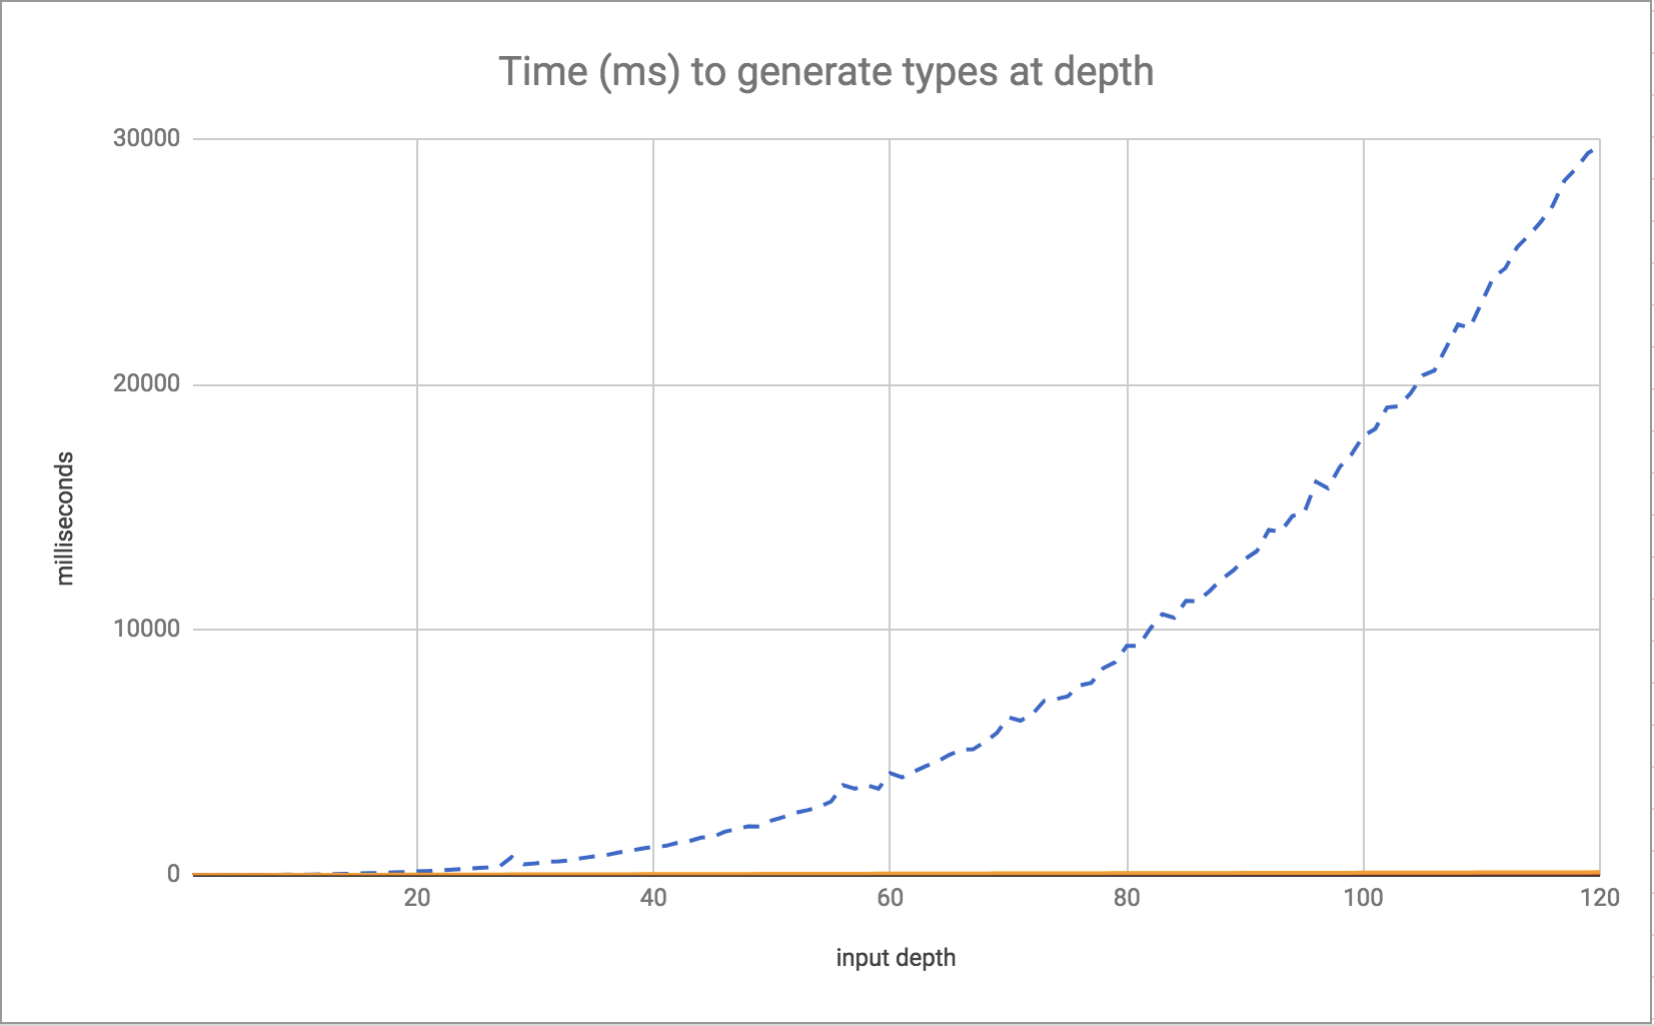
\includegraphics[width=\textwidth]{tagged-untagged-depth-bench120}

Benchmark 1 is represented by the red solid line, benchmark 2 by the
blue dotted line.

The graph shows the performance of Benchmark 1 is constant, because
the width of the largest union is always 2\ in an early phase of the reconstruction
algorithm.

The results for Benchmark 2 show the reconstruction algorithm is quadratic
with respect to the size of the largest union.

These observations are consistent with the prior theoretical analysis.

\Dsection{Can space use be bounded by reducing traces as collected?}

Traces in Typed Clojure's dynamic analysis are accumulated online, and then
folded into a type environment offline. However, this fold operation is commutative
with respect to the order of traces, so performing this fold online would
eliminate the need to store traces in memory.

Space is reduced further, then, by leveraging \texttt{join} to eagerly simplify
the accumulated type environment. For example, heterogeneous maps with similar
keysets could merged, possibily using optional key entries, saving space by
preventing very large redundant unions.

It is unclear if it is possible to perform more sophisticated analyses online,
in particular the recursive type reconstruction algorithm. Since the resulting
annotations are very compressed compared to intermediate points in the analysis,
fully or partially performing this analysis online may drastically decrease space
usage where recursively defined maps are used, and very deep examples are found.

\Dsection{Comparison to Daikon}

Daikon is a related system to Typed Clojure's dynamic type inference.
However, Daikon is built for ``invariant detection'', while our system
is designed for ``dynamic type inference'' or ``value profiling''.

There are two common implementation strategies for such tools. The first
strategy, ``ruling-out'' (for invariant detection), assumes all invariants are true 
and then use runtime analysis results to rule out
impossible invariants. The second ``building-up'' strategy (for dynamic type inference)
assumes nothing and then uses runtime analysis results to build up invariant/type knowledge.

Both strategies have different space behavior with respect to representing
the set of known invariants.
The ruling-out strategy typically uses a lot of memory at the beginning,
but then can free memory as it rules out invariants. For example, if
\texttt{odd(x)} and \texttt{even(x)} are assumed, observing \texttt{x = 1}
means we can delete and free the memory recording \texttt{even(x)}.
Alternatively, the building-up strategy uses the least memory storing
known invariants/types at the beginning, but increases memory usage
as more the more samples are collected. For example, if we know
\texttt{x : Bottom}, and we observe \texttt{x = "a"} and \texttt{x = 1}
at different points in the program, we must use more memory to
store the union \texttt{x : String $\cup$ Integer} in our set of known invariants.

Examples of invariant detection tools include Daikon \cite{Ernst06thedaikon},
DIDUCE \cite{hangal2002tracking}, and Carrot \cite{pytlik2003automated}, and
typically enhance statically typed languages with more expressive types or contracts.
Examples of dynamic type inference include Rubydust \cite{An10dynamicinference},
JSTrace \cite{saftoiu2010jstrace}, and TypeDevil \cite{pradel2015typedevil},
and typically target untyped languages.

%There is some overlap between invariant detection and dynamic type inference
%tools. Usually, invariant detection detects very expressive relationships
%between program variables; for example, for array \texttt{a} and index
%\texttt{i} variables, a derived invariant might be \texttt{0 < a[i]}.
%On the other hand, dynamic type inference (or value profiling) often just records
%basic nominal or structural type information---it is generally applied to untyped
%languages where basic static type information is absent.

\Dsubsection{Daikon's expressivity vs Typed Clojure's dynamic inference}

Daikon can reason about very expressive relationships between variables
using properties like ordering ($x < y$), linear relationships ($y = ax + b$),
and containment ($x \in y$). It also supports reasoning with ``derived variables''
like fields ($x.f$), and array accesses ($a[i]$).

Typed Clojure's dynamic inference can record heterogeneous data structures
like vectors and hash-maps, but otherwise cannot express relationships
between variables.

There are several reasons for this. The most prominent is that Daikon
primarily targets Java-like languages, so inferring simple type information
would be redundant with the explicit typing disciplines of these languages.
On the other hand, the process of moving from Clojure to Typed Clojure
mostly involves writing simple type signatures without dependencies
between variables. Typed Clojure recovers relevant dependent information
via occurrence typing, and gives the option to manually annotate necessary
dependencies in function signatures when needed.

\Dsubsection{Space/time overhead of Daikon's dynamic tracing}

Performance of dynamic tracing is not directly addressed in the Daikon
literature, who only provide complexity analyses and optimizations for storing
and checking invariants \emph{after} samples have been collected.

I have manually examined Chicory (the Java front-end to Daikon) to see how
dynamic tracing is implemented.
I found that Daikon records the value of all variables in scope
at each method entry/exit point \footnote{Implemented in \texttt{daikon.chicory.DaikonVariableInfo}}.
Then, to record values in Daikon, the following algorithm is used:

\begin{itemize}
  \item If the value is a Java primitive, record its value.
  \item If the value is an array, traverse its contents and record identity hash codes
    and/or primitive values.
  \item Otherwise, record the class of the current object.
\end{itemize}

Notice this algorithm is non-recursive---while arrays are traversed eagerly, they
are only traversed one level via an identity hash code summary (the closest equivalent to
pointer addresses on the JVM).
This is significantly different to Typed Clojure's value tracing algorithm,
which recursively (but lazily) traverses potentially-deep data structures.

Another difference is that Typed Clojure's dynamic tracing only tracks
values for arguments/returns of a function, and ignores any variables
that in are scope. There are several reasons behind this decision.
First, Java-like object-oriented languages use fields as implicit
arguments to methods, and Daikon distinguishes method-level, and class-level
invariants which is achieved by checking class-level invariants during
method calls.
In Clojure, methods are replaced with pure functions (their output is defined only by the
explicitly passed arguments), so the method/class-level distinction is
not applicable.

Second, Daikon chooses to reason about local mutation in Java-like languages,
and so must record the values of the same variables different program points
to observe mutation. However, local unsynchronized mutation is non-idiomatic
in Clojure so re-tracking variables is almost always redundant---mutation is
often via synchronized global variables that can be instrumented once-and-for-all.

\Dsubsection{Space/time overhead of Daikon's type inference}

The overhead of likely invariant detection
is described by Perkins and Ernst~\cite{Perkins04efficientincremental}.
They analyze the overhead of storing and checking the set of
invariants that are currently true.
Their presentation includes a simple incremental algorithm that
features no optimizations, then they propose several candidate
optimizations and empirically compare the performance of each
approach.

The space complexity of the simple incremental algorithm is dominated 
by the size of the grammar of properties. For example, if the grammar
of properties consists of $=$ and $even$, with
3 variables $x$, $y$, $z$, the initial (and largest) set of invariant assumptions
is $x = y$, $y = z$, $x = z$, $even(x)$, $even(y)$, and $even(z)$.
For reference, Daikon enables 152 properties by default, with
12 ``derived variables'', the latter of which provide properties on composite variables
like $a[x] = a[z]$. After a static analysis pass ruling out nonsensical invariants,
the space usage is at least $O(v^9)$, where $v$ is the number of variables in scope.

The time complexity of \emph{checking} invariants for each sample
is similarly dominated by the size of the grammar of properties.
They note, however, most invariants are removed quickly (after
$O(1)$ samples), so performance improves as more samples
are collected.

\Dsubsection{Checking Daikon's invariants in a refinement type system}

Daikon has expressive invariants, but can they be statically verified?
Yes, in fact Daikon supports generating annotations for a Java-based
theorem prover called Simplify~\cite{Detlefs03simplifya}.

Simplify implements the following theories.

1. The theory of equality, \texttt{=}

2. The theory of arithmetic with functions \texttt{+}, \texttt{*}, \texttt{-},
   and relation symbols \texttt{>}, \texttt{<}, \texttt{<=}, and \texttt{>=}.

3. The theory of maps with two functions \texttt{select} and \texttt{store} (ie. get/set),
   and two additional axoims.

4. Partial orders. % (?)

These could be encoded in Dependent Typed Racket, since it supports propositions
in linear arithmetic constraints about variables, pairs, car, and cdr.

% Notes:
%  Java implementation:
%    Chicory does instrumentation on JVM bytecode
%     instrument_all_methods: https://github.com/codespecs/daikon/blob/master/java/daikon/chicory/Instrument.java#L409
%      add_entry_instrumentation
%     - https://github.com/codespecs/daikon/blob/master/java/daikon/chicory/Instrument.java#L825
%      add_return_instrumentation
%       - instruments return statements
%      - https://github.com/codespecs/daikon/blob/master/java/daikon/chicory/Instrument.java#L675
%     daikon.chicory.Runtime
%      - contains wrappers for values that are rewritten to?
%      - Runtime.enter(...) is called at the top of every wrapped method
%      - `dtrace_writer` records inference results
%      daikon.chicory.DaikonVariableInfo
%      - actually traverses values here
%      - arrays are traversed eagerly, but only one level
%        - subsequent levels use identityHashCode summaries



\appendix
%\section{Appendix Title}
%\subsection{math.combinatorics}
%
%Problems:
%
%\begin{itemize}
%  \item hard to annotate
%  \item overly dynamic idioms
%  \item polymorphism
%\end{itemize}
%
%\begin{verbatim}
%Issues
%- (partial map v)
%  - too hard to infer
%- #(map v %) has no annotation generation
%- (apply concat ...) not inferring
%- permutations should be polymorphic
%- sorted-number? should infer a :then filter of (Coll Num)
%- `reductions` needs annotation
%- (every? seq ...) should generate good filter
%- many things should be polymorphic
%\end{verbatim}

\bibliography{bibliography}

\end{document}
